\chapter{Higgs Decay to Two Photons}

The two photon channel is one of the most promising decay modes in the search for the SM Higgs
at the LHC. Despite having a relatively small branching ratio, the decay $\Hgg$ 
provides a very clean, fully reconstructible final-state topology making it 
one of the most sensitive channels at low mass.
The dominant source of background is from real, prompt diphoton events from QCD 
processes, $pp\rightarrow\gamma\gamma$ (prompt-prompt).
In addition, there is a contribution from $pp\rightarrow\gamma+jet$ (prompt-fake) and 
$pp\rightarrow jet+jet$ (fake-fake) in which jets are mis-identified as photons. 
As the signal rate in the $\Hgg$ decay is expected to be small compared to the background rates,
the search sensitivity is heavily influenced by how well the backgrounds are understood.
For this reason, two data-driven background modelling techniques were developed
The first uses a fully parametric
description of the background from data designed to incorporate systematic uncertainties as additional degrees of 
freedom in its functional form~\cite{HIG-11-033}. The second uses a binned model constructed from 
sidebands in the $\mgg$ spectrum. The latter of these two serves as an independent cross-check of the former,
in particular by allowing direct inclusion of the systematic uncertainties in the signal extraction thereby
building confidence in the understanding of the background. 
This chapter describes a search for a Higgs boson decaying to two photons
which was performed on the full 2011 dataset corresponding to \clumi of proton-proton collisions 
recorded at CMS at a center of mass energy of 7 TeV.

\section{Data Samples}
\label{sec:datasamples}

The dataset used for this analysis is the combination of the 2011A and 2011B 
proton-proton collision runs.
The selection for the dataset used for this analysis is based around dedicated diphoton triggers
which select events online which satisfy one of two sets of criteria.
The first set requires two HLT photon candidates, one with $\pt>26$ GeV and the other with 
$\pt>18$ GeV, which are well isolated in the calorimeter~\cite{AN-12-048}. The second has a lower threshold on
the first photon, $\pt>22$ GeV but requires that both photons have localised showers in the ECAL 
($\rnine>0.8$ in 2011A and $\rnine>0.9$ in 2011B). 
Additionally, the invariant mass of the two trigger objects are required to have an 
invariant mass greater than 60 (70) GeV in the 2011A(B) datasets.
Events which would pass the full offline selection but failed to trigger at the HLT lead to an inefficiency, 
reducing the number of signal events with respect to that expected from an integrated luminosity of \clumi.
However, the thresholds applied offline are chosen to be much tighter than those of the trigger;
the trigger efficiency is $>$99\% with respect to the analysis selection~\cite{AN-12-048}. 

Signal Monte Carlo (MC) events are generated for a Higgs decaying to two photons via the four main 
production processes, gluon-gluon fusion ($ggH$), vector boson fusion ($qqH$) and associated $W/Z$ ($VH$) 
and $\ttbar$ ($ttH$) production.
The gluon-gluon fusion and vector boson fusion were generated with \texttt{POWHEG}~\cite{powheg} with 
next-to leading order (NLO) contributions whereas
the two associated production processes were generated to leading order (LO) only.
The $\pt$ spectrum of the Higgs ($\pt^{H}$) from gluon-gluon fusion was calculated at
next-to-next-to leading plus next-to leading log resummed order (NNLO+NLL) using the \texttt{HqT} program~\cite{hqt}.
The production cross-sections and branching ratios are taken from the LHC Cross-section Working Group~\cite{lhcxswg}.

MC for background processes were generated at LO using \texttt{POWHEG} interfaced with \texttt{PYTHIA}~\cite{pythia}.
The QCD dijet and $\gamma+jet$ samples are filtered by requiring the generated photons, electrons and neutral
mesons with $\pt>15$ GeV have at most one charged particle in a cone, $\Delta R<0.2$, to increase the 
production efficiency with respect to the tracker isolation requirements of the full selection.
The background samples considered for this analysis are summarized in Table~\ref{tab:backgroundmc}.
A full simulation of the CMS detector is provided in \texttt{GEANT4} which is used for all signal
and background MC samples~\cite{geant4}. The MC includes a simulation of additional interaction vertices expected in data
from pileup. The distribution in the number of reconstructed vertices in MC  is corrected to match that observed
in data as described in Section~\ref{sec:pileup}.

\begin{table}
\begin{center}
\begin{tabular}{|l r|c|c|}
\hline
\textbf{Process}  & &  \textbf{Cross-section} ($pb$) & \textbf{Luminosity} ($pb^{-1}$)\\
\hline
\hline
DiPhotonJets & & 154.7 & 7400 \\
\hline
DiPhoton Box & $\hat{\pt}~25-250$ & 12.37 & 41900 \\
\hline 
QCD Dijet    & $\hat{\pt}~30-40$      & 10870 & 560 \\
	     & $\hat{\pt}~40-\infty$  & 43571 & 920 \\
\hline 
Gamma+Jet    & $\hat{\pt}~20-\infty$  & 493.44& 2400 \\
\hline 
DrellYan+Jets to $ll$  & $\hat{\pt}~50-\infty$  & 2475& 14000 \\
\hline
\end{tabular}
\caption{Background MC used throughput the analysis with production cross-sections and 
corresponding equivalent integrated luminosity.}
\label{tab:backgroundmc}
\end{center}
\end{table}


\section{Object Reconstruction and Identification}
\label{sec:objectrecoandid}

The reconstruction of all objects used for this analysis, in both data and MC,
is based on the standardized CMS reconstruction software \texttt{\cmssw}~\cite{null}. 
Additional sensitivity can be gained by refining the object selection and reconstruction specifically
to the search for $\Hgg$.

\subsection{Supercluster Energy Correction}
\label{superclusterenergyreconstruction}

As the natural width of Higgs boson is around 100 MeV, the width of a reconstructed mass peak from 
a $\Hgg$ decay is driven by the experimental energy resolution of the photons.
This resolution can be improved dramatically by correcting the raw energy of the supercluster 
on a per-photon level. These corrections are derived using a multivariate technique 
in which a regression BDT is trained on prompt photons in the gamma+jet MC sample using the 
ratio of the generated photon energy to the raw energy of the reconstructed supercluster.
As this ratio can vary across different regions of the detector, the input variables include both the 
$\eta$ and $\phi$ positions of the supercluster. In addition, several variables are included which 
describe the shower shape: $\rnine$, the energy weighted widths in $\eta$ and $\phi$ of the supercluster,
the energy weighted crystal width ($\sigieie$) and the ratio of hadronic energy behind the supercluster
to the energy of the supercluster itself ($\hoe$). In the endcaps, there is additional information 
available from the pre-shower measurement. The ratio of the energy in the pre-shower to the raw supercluster energy
is included for superclusters in the ECAL endcaps. Figure~\ref{fig:mcregrcomparison} shows the improvement
in resolution after applying the regression corrections compared to the raw measurement.
In addition, a similar set of corrections were derived using by fitting an analytical expression 
of the residual energy difference between the 
generated and reconstructed photon energy as a funciton of supercluster energy, position and $\rnine$~\cite{AN-11-343}. 
The regression technique reduces the effective resolution of the Higgs mass peak ($\sigma_{eff}$) 
resolution by around 30\% over using the raw supercluster energy compared to the analytic fit which
improves the resolution by 15\%. 

\begin{figure}
\begin{center}
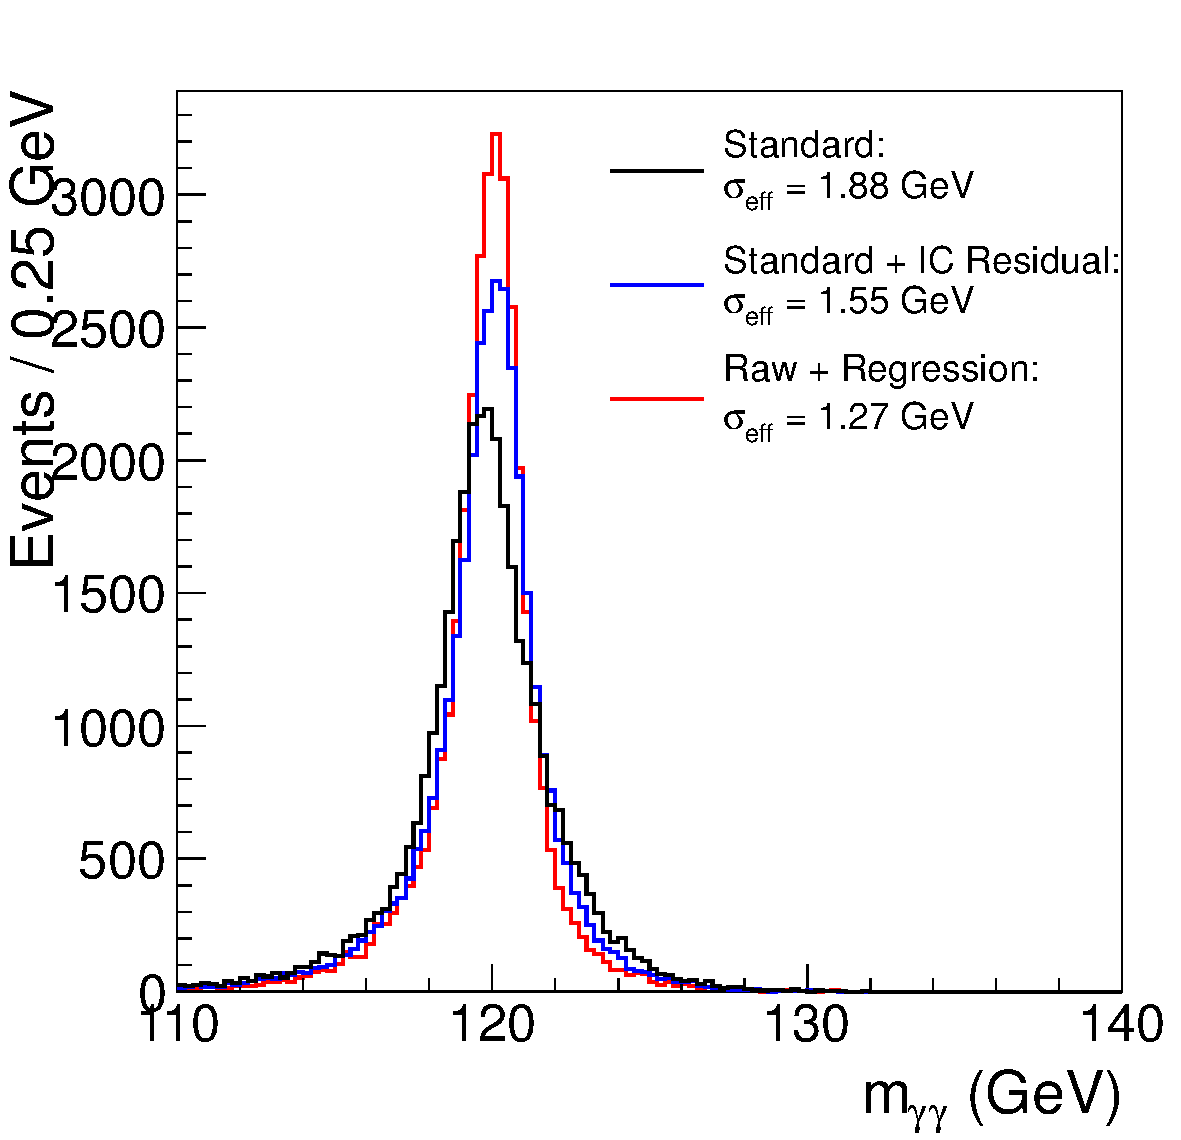
\includegraphics[width=.6\textwidth]{hgg7TeV/generalPlots/regrresall.pdf}
\label{fig:mcregrcomparison}
\caption{Comparison of the diphoton mass peak in MC Higgs with a mass of 120 GeV using different 
measurements of the photon energy. The black line 
is from using the raw energy of the supercluster, the blue is from using the analytic fit method 
and the red from using the regresssion method. The quantity $\sigma_{eff}$,
the narrowest range in $\mgg$ which contains 68\% of the distribution, is given for each peak.}
\end{center}
\end{figure}

An estimate of the per-photon energy resolution, $\sigma_{E}$, is obtained by training a second 
regression BDT targeting the absolute deviation between the correction estimated by the 
first BDT and the true correction to generator level. This second BDT is trained on an independent
set of events to the first. The per-photon resolution is used to calculated an estimate of the 
per-event mass resolution, $\sigma_{\mgg}$, which is used during the event selection 
(Section~\ref{sec:eventselection}). An additional regression BDT is trained on $\Zee$ MC which is used
to compare the supercluster energy scale in data and MC~\cite{AN-12-048}.

\subsubsection{Energy Scale Measured in Data}
Despite correcting the energy of the photons using the regression technique, discrepancies between data and
MC are still observed. This is due to additional detector effects which may not be simulated, such as the
time dependence of the ECAL crystal transparency~\cite{null}. Further corrections are
derived based on $\Zee$ events which provide an invariant mass peak with almost no background constructed from 
electromagnetic objects which are reconstructed using a similar procedure to photons.
The energy scale of the superclusters is measured by matching the electron
invariant mass peak in data to that in MC. This is achieved using an analytic fit to the $\Zee$ peak in data and MC
separately. The natural peak of the $Z$ is described using a Breit-Wigner distribution whose parameters are fixed
to those given by the Particle Data Group, $m_{Z}=91.188,~\Gamma_{Z} = 2.495$~\cite{pdg}. This is then convoluted 
with a Crystal Ball (CB) which describes the resolution effects of the calorimeter and energy losses from 
bremsstrahlung before the ECAL~\cite{crystalball}. 
The CB parameter $\Delta m$ is a free parameter of the fit giving the 
offset of the peak position from the $Z$ pole. 

The values of these fitted parameters varies with the position of the supercluster ($|\eta|$). Moreover the
variation in data is strongly dependant on the run during which the data were taken. The scale is extracted in 
six run ranges and four $|\eta|$ regions to account for this effect. 
The difference between MC and data with time is less dependant on whether the electron showered or not which 
is characterised by the $\rnine$ of the supercluster. The data-MC difference in each $|\eta|$ region is measured
a second time after applying the first set of corrections to the data and obtaining the residual difference
for electrons with $\rnine<0.94$ and $\rnine>0.94$ separately. The final energy scale correction is then defined
as the product of the two corrections. The relative correction, 

\begin{equation}
1-\Delta P = 1 - \frac {\displaystyle \Delta m_{data} - \Delta m_{MC} }{\displaystyle m_{Z} }
\end{equation}

is applied to the photons in data. The values for the scale in each category, $\Delta P$, are given in 
Table~\ref{tab:escale2011}. The uncertainties on these measurements are primarily due to 
the difference in the $\rnine$ distribution of electrons and photons. In addition, smaller systematics
are included due to the variation of the measurements when changing the electron selection and
between using the electron-trained and photon-trained regression corrections.
These uncertainties are incorporated into the signal model for the purposes of 
signal extraction as described in Section~\ref{sec:signalmodel}.

\subsection{Vertex Selection}
\label{sec:vertexselection}

The assignment of the correct vertex to the diphoton pair is an important step in the reconstruction of 
its invariant mass. Since photons do not leave tracks, computing the angle between the two photons 
depends strongly on determining the interaction in which they were produced.
Figure~\ref{fig:higgsrightwrongvertex} shows the invariant mass distributions from a SM
Higgs boson for events in which the vertex selected is within 10mm of the generated vertex
compared to those in which an incorrect vertex is assigned. 

\begin{figure}
\begin{center}
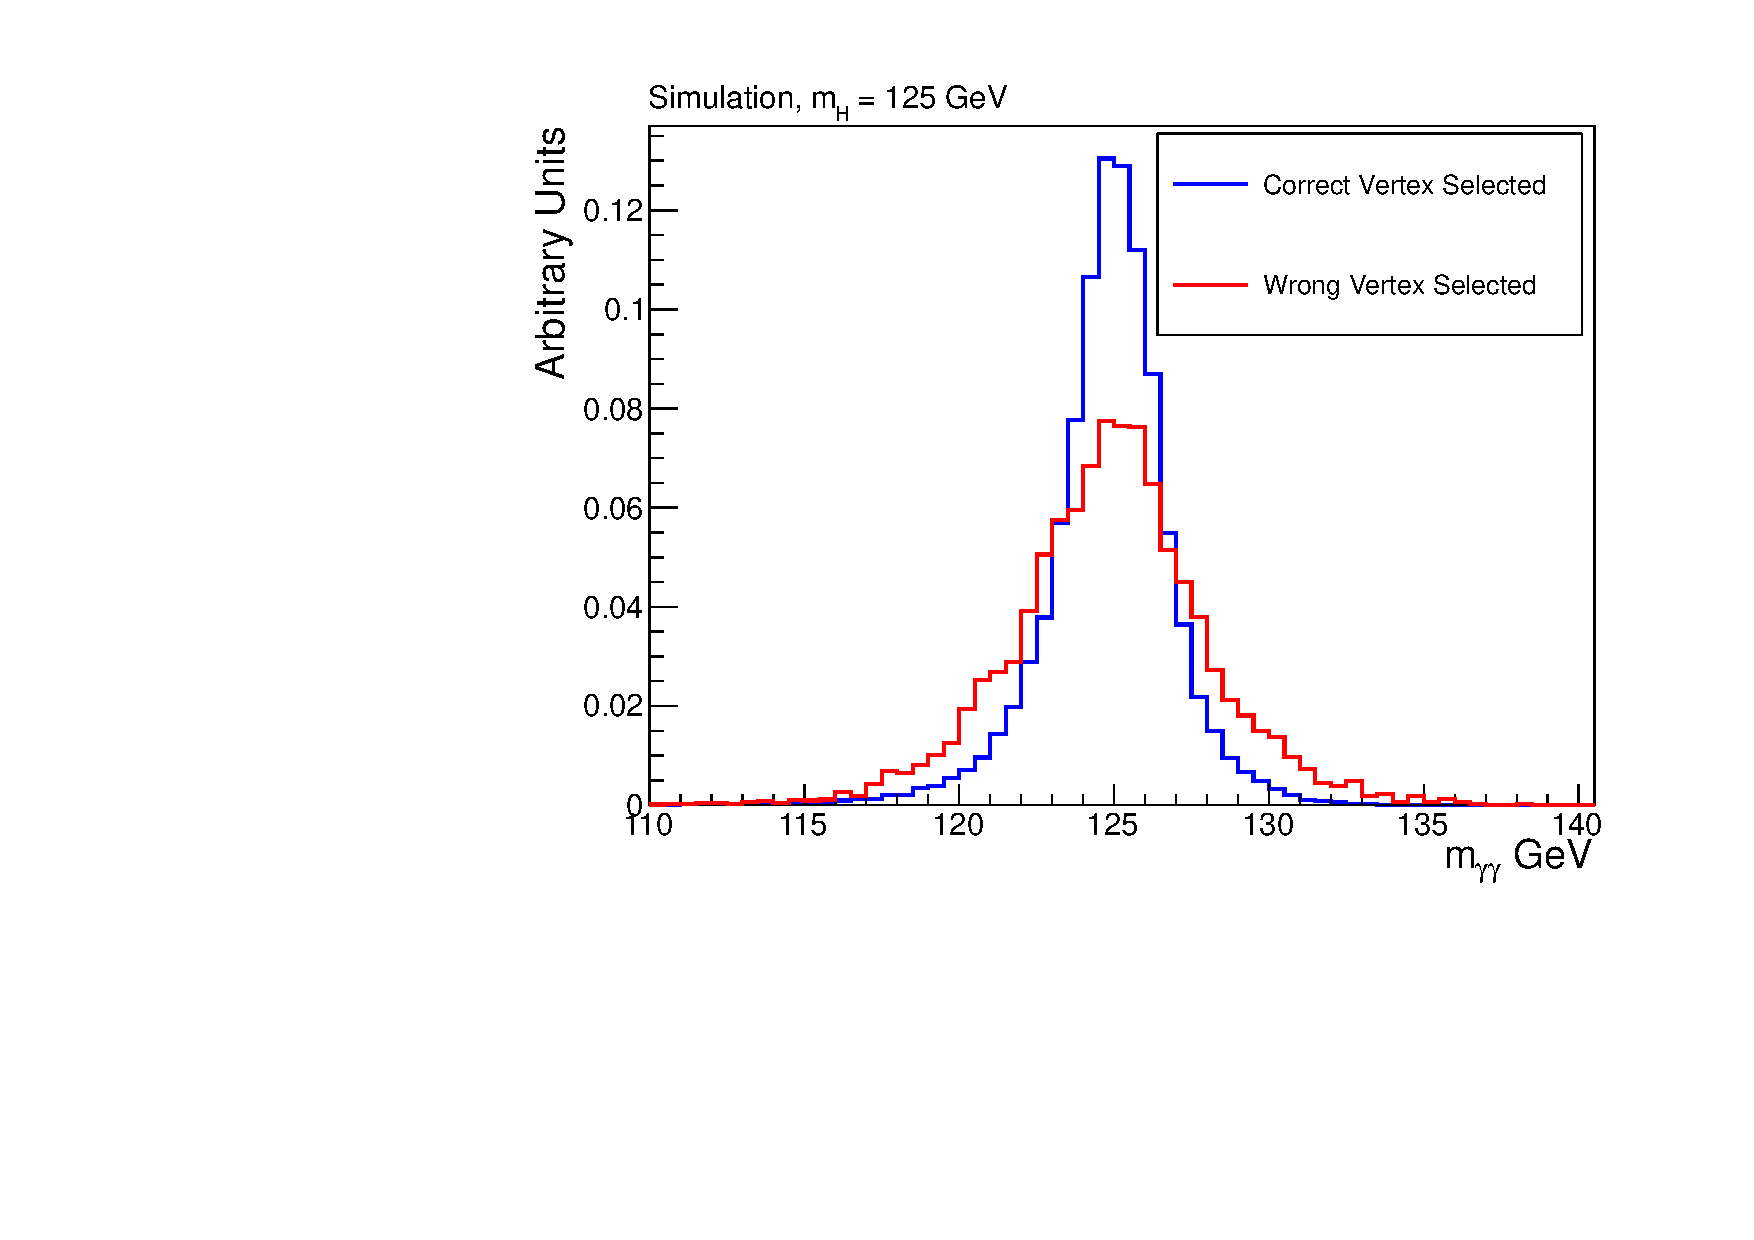
\includegraphics[width=.8\textwidth]{hgg7TeV/generalPlots/rightwrongvtxpeak.pdf}
\label{fig:higgsrightwrongvertex}
\caption{Invariant mass peak in $\Hgg$ MC with mass 125 GeV. The blue histogram is from events in which 
the generated vertex is within 10mm of the vertex assigned to the diphoton pair. The red histogram is 
from events in which the incorrect vertex is assigned. Both distributions are normalised to unit area for
ease of comparison.}
\end{center}
\end{figure} 

A BDT was trained to rank the standard collection of reconstructed vertices.
The input variables are chosen to exploit the correlation between the diphoton system and the recoiling tracks.
These are the $\pt$-balance and $\pt$-asymmetry calculated as,

\begin{eqnarray}
	-\sum_{all tracks} \left(\ptvec^{track}\cdot \frac{\displaystyle \ptggvec}{\displaystyle \ptgg}\right) 
\end{eqnarray}
and
\begin{eqnarray}
	\frac{\displaystyle |\sum_{all tracks} \ptvec^{track}| - \ptgg }{ \displaystyle|\sum_{all tracks} \ptvec^{track}|} 
\end{eqnarray}

respectively. In addition, the sum of the square of the transverse momenta of all the tracks associated 
to a given vertex is included to preferentially select hard interactions. If at least one of the 
photons converts to an $e^{+}e^{-}$ pair, the difference between the position in $z$ as calculated 
using the electron-positron pair and that from the standard vertex, relative to the resolution in $z$
is included as an input variable. The BDT was trained on $\Hgg$ MC with a mass of 120 GeV. 
Figure~\ref{fig:vtxeffhmc} shows the fraction of events in a gluon-gluon MC sample in which 
the vertex with the highest BDT score is within 10mm of the true vertex as a function of $\pt^{H}$.

\begin{figure}
\begin{center}
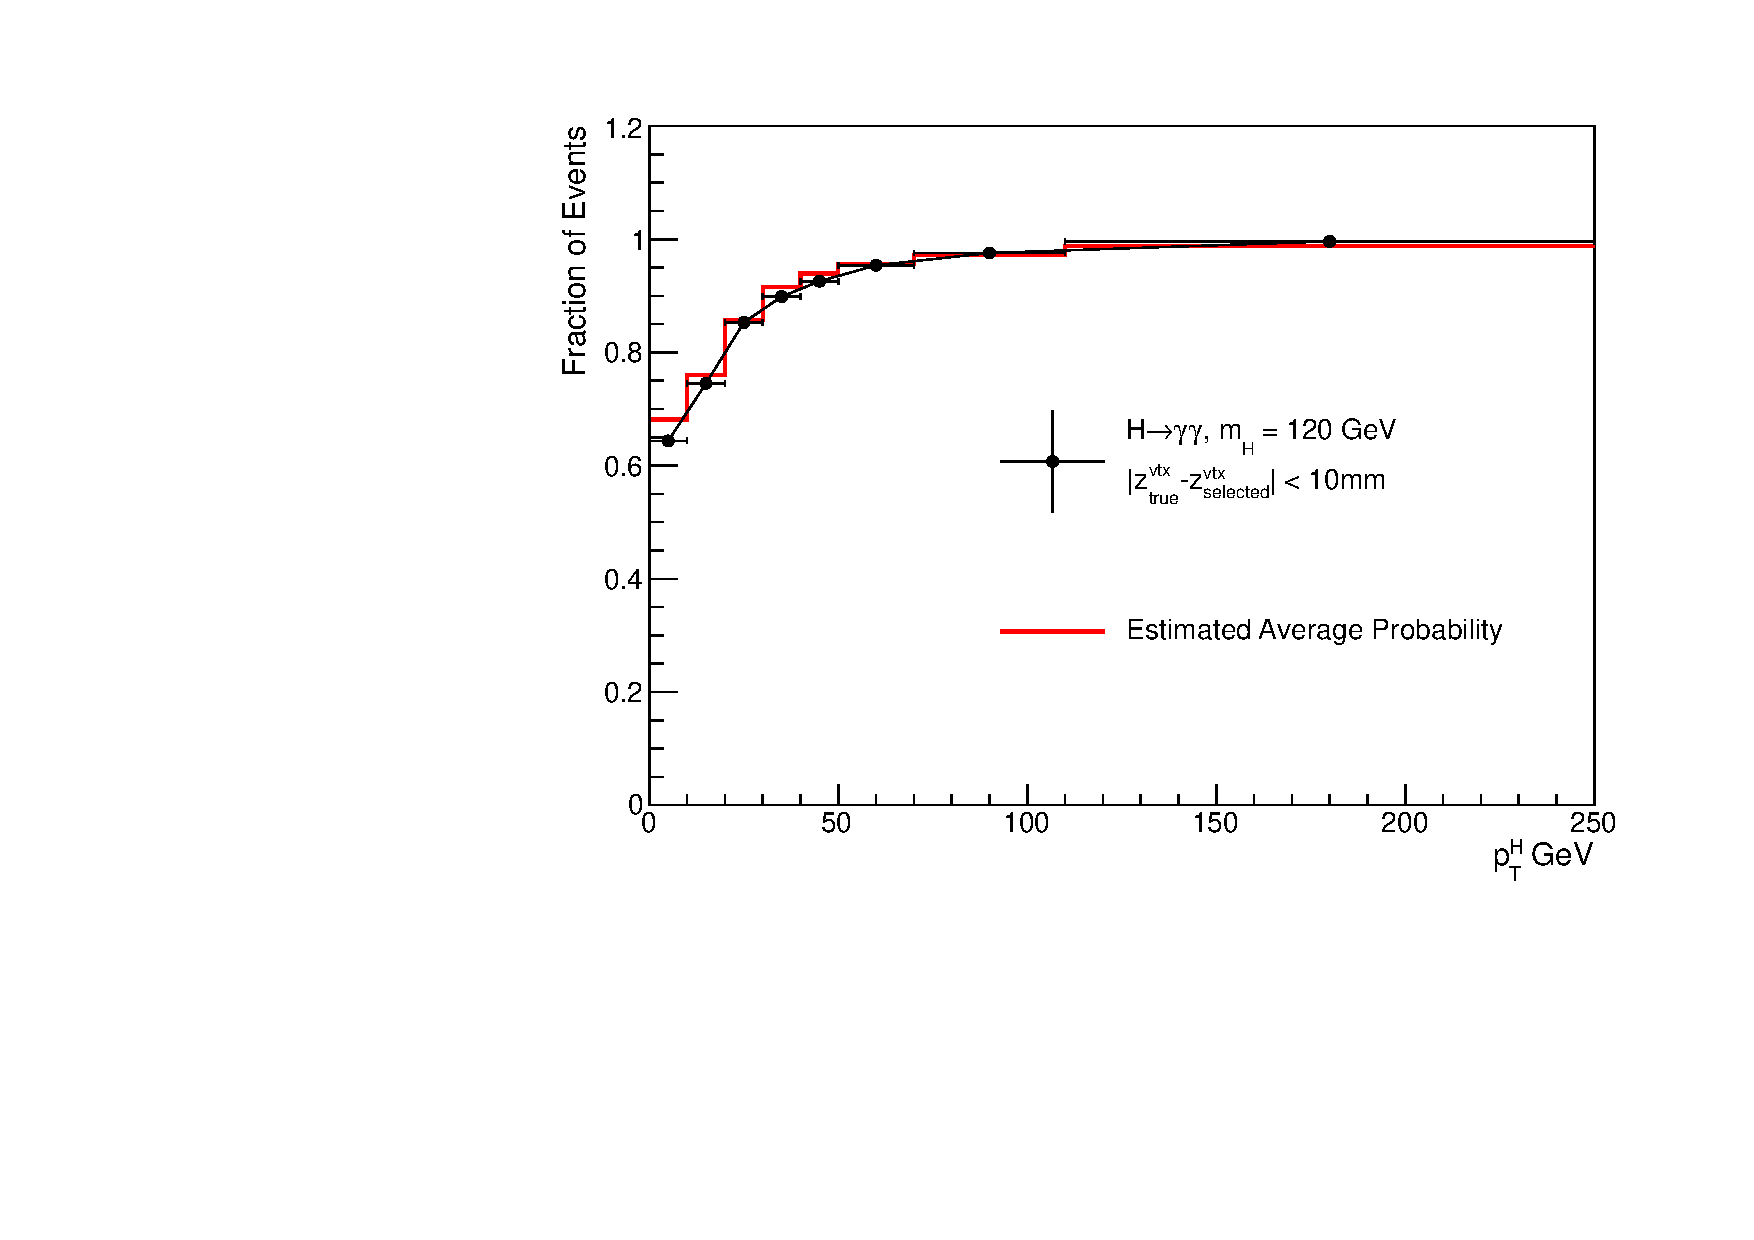
\includegraphics[width=.8\textwidth]{hgg7TeV/generalPlots/vtxEffHMC.pdf}
\label{fig:vtxeffhmc}
\caption{Fraction of simulated gluon-gluon fusion events in which the selected vertex $z$ position 
is within 10mm of the true vertex as a function of Higgs $\pt$. The red histogram is the average 
probability to select the correct vertex in each bin estimated from the per-event BDT.}
\end{center}
\end{figure} 

The fraction of events in which this occurs in data is measured using $\Zmumu$ events
as a function of the $\pt$ of the $Z$ boson~\ref{AN-11-048}. This is used to correct the Higgs signal MC for 
the purpose of signal modelling. A second, per-event BDT is trained using the output of the first, to identify 
under which conditions the correct vertex is selected. The output of this BDT is then used to 
calculate the probability in a given event that the correct vertex is assigned. The red line in Figure~\ref{fig:vtxeffhmc}
shows a comparison of the per-event vertex probability estimated from the second BDT against the 
fraction of the events in which the selected vertex is located within 10mm from the true vertex.

\subsection{Photon Identification}
\label{sec:photonidentification}

A large portion of the fake background in the $\Hgg$ search is due to high momentum neutral mesons
which decay to two photons where both the photons are combined into the same supercluster~\cite{HIG-12-015}. 
Information from the shower shape of the photon supercluster can be used, in addition to the 
energy isolation within the calorimeter, in order to distinguish these from prompt photons
from the primary interaction point. A BDT was trained on MC events to combine the relevant information
into a single photon identification (ID) discriminator. The signal used for the training was taken from 
simulated $\Hgg$ events with a Higgs boson mass of 121 GeV while the background was 
taken from non-prompt photons in the Gamma+Jet sample.
Before training, events are required to pass a loose preselection designed to avoid training 
where the MC is unable to properly describe the data and to match the variables used in the trigger~\cite{AN-12-048}.
In addition, photon candidates are removed if there is a reconstructed \texttt{GsfElectron} matched to the 
photon supercluster with no matching conversion reconstruction. This greatly reduces the contribution
from $\Zee$ faking photons. The same preselection is applied to all MC and data for extracting the signal.
The efficiency of the preselection for signal was measured in $\Zee$ data and MC using a tag-and-probe 
method~\cite{AN-12-116}. The results are shown in Table~\ref{tab:sigeffpresel}. 

\begin{table}
\begin{center}
\begin{tabular}{| l | c | c | c |}
\hline
\textbf{Category} & \textbf{Data} & \textbf{MC} & \textbf{Data/MC} \\
\hline
EB $\rnine>0.9$ & 0.9267 $\pm$ 0.0012 & 0.9275 $\pm$ 0.0006 &0.999 $\pm$ 0.0013 \\
EB $\rnine<0.9$ & 0.8882 $\pm$ 0.0023 & 0.9025 $\pm$ 0.0010 &0.984 $\pm$ 0.0025 \\
EE $\rnine>0.9$ & 0.9442 $\pm$ 0.0010 & 0.9387 $\pm$ 0.0009 &1.006 $\pm$ 0.0014 \\
EE $\rnine<0.9$ & 0.8639 $\pm$ 0.0010 & 0.8517 $\pm$ 0.0011 &1.014 $\pm$ 0.0015 \\
\hline
\end{tabular}
\caption{Signal efficiency for the preselection measured in data and MC using tag-and-probe in
$\Zee$ events. The ratio Data/MC are applied as corrections to the signal MC for the purposes
of signal modelling. The uncertainties listed here are statistical only.}
\label{tab:sigeffpresel}
\end{center}
\end{table}

The input variables are chosen to be insensitive to the kinematics of the diphoton system itself
including the diphoton invariant mass. The first set of variables describe the shower shape of the 
supercluster: $\hoe$, $\sigieie$, $\rnine$ and the energy weighted widths of the supercluster in
$\eta$ and $\phi$ ($\sigma_{\eta},~\sigma_{\phi}$). The $\eta$ of the supercluster is 
included as the shower shape is dependant on the position within the calorimeter. 
The second set of input variables describe the
isolation of the photon in the calorimeter and tracker scaled to account for 
the additional expected energy density due to pileup, $\rho$~\cite{2011JInst611002C}. 
These are the sum of the track isolation, 
calculated relative to the chosen vertex and the vertex giving the maximum track isolation,
ECAL isolation and HCAL isolation in a cone with $\Delta R<0.3$ minus $\rho$ times the effective area 
of the cone~\cite{2011JInst611002C}.
and the absolute ECAL and HCAL isolations within cones of $\Delta R <0.3$ and $\Delta R<0.4$ 
respectively. In addition, the number of reconstructed vertices in the bunch crossing is included
to reduce the pileup dependence of the isolation variables. 

A separate BDT is trained for application in the ECAL barrel and endcaps as the shower
shape and isolation variables are rather distinct between the two components. 
A cut is made on the photon ID BDT output to select events used for the signal extraction which
keeps practically all ($>99\%$) of the signal while removing around 22\% of background events.
The cut is chosen to be loose as the output of the photon ID will be used as input for the 
event selection (diphoton BDT) as described in Section~\ref{sec:diphotonbdt}. 

\section{Event Selection}
\label{sec:eventselection}

In addition to passing the preselection, the two photons are required to pass mass-dependant transverse 
momenta cuts, $p_{T}/\mgg > 1/3, ~1/4$ for the leading and subleading photon respectively.
Where more than one diphoton pair satisfies these criteria in an event, the pair which has the largest
sum of photon transverse momenta is selected as the Higgs candidate.
The final selection of diphoton candidates used for the signal extraction is based on using as much information 
in the event as possible to distinguish likely signal candidate events from the background. Although the 
photon ID BDT is successful at rejecting fake backgrounds, a large portion of the background is due to
real prompt diphotons from QCD processes. In order to distinguish these from a Higgs signal, 
the specific kinematics and topology of the event are exploited.

\subsection{Diphoton BDT}
\label{sec:diphotonbdt}
A BDT was trained to utilise the kinematics of the selected diphoton pair to discrimiate prompt photons
from QCD background from those produced by the decay $\Hgg$. The BDT was trained using the QCD Dijet,
Gamma+Jet, DiphotonJets and Diphoton Born samples for background and Higgs MC with a mass of 123 GeV.
As the mass of the Higgs boson is unkown, the search is performed under different mass hypotheses.
In order to allow for the application of the same selection to the data under any mass hypothesis,
the input variables to the BDT are chosen to be mass-independant. In addition, this allows
for a fully data-driven estimation of the background shape as described in Section~\ref{sec:backgroundmodel}.
The input variables which describe the kinematics are:
the relative transverse momenta of the photons, $\pt^{1},~\pt^{2}$, 
their pseudo-rapidites, $\eta^{1},~\eta^{2}$ and the cosine of the 
angle between the two photons in the transverse plane $cos(\Delta\phi)=cos(\phi^{1}-\phi^{2})$.
In addition, information regarding the quality
of the objects, the two photons and the selected vertex, is included in the form of the output of the 
photon ID and the vertex probability. The per-photon resolution estimate, $\sigma_{E}$ is combined for
each photon to produce a per-event mass resolution estimate ($\sigma_{\mgg}$) under the assumption that 
the correct vertex is selected;

\begin{equation}
\sigma_{\mgg} (right-vtx) = \frac{\displaystyle \mgg}{\displaystyle 2} 
\sqrt{ \left( \frac{\displaystyle {\sigma_{E}^{1}}}{\displaystyle E^{1} } \right)^{2}
     + \left( \frac{\displaystyle {\sigma_{E}^{2}}}{\displaystyle E^{2} } \right)^{2}
     }
\end{equation}
where $E^{1},~E^{2}$ are the energies of the two photons.

Since the correct vertex is not always selected, the mass resolution assuming the incorrect vertex is chosen
is calculated using the average beamspot length in data, $\sigma_{Z}=5.8$cm. In this case, the distance 
between the selected and true vertex will be distributed as a Gaussian with width $\sqrt{2}\sigma_{Z}$.
The contribution to the resolution, $\sigma_{\mgg}^{vtx}$, can be calculated analystically given the positions of
the two photons. The mass resolution estimator under the assumption that the incorrect vertex is chosen is 
given by the sum in quadrature of $\sigma_{\mgg}^{vtx}$ with the mass resolution assuming the correct vertex is chosen.
Both estimators for the mass resolution relative to the invariant mass, $\sigma_{\mgg}/\mgg~$ right/wrong-vtx, 
are included as inputs to the diphoton BDT. Figure~\ref{fig:diphotonBDT} shows the diphoton BDT distribution in 
data and MC. In addition to further separating the contribution to the background from fakes, the diphoton BDT 
can discriminate between prompt diphotons in QCD and those from a $\Hgg$ decay. The final events used for 
the signal extraction are selected as those with a diphoton BDT output greater than 0.05. This cut is chosen
following an optimization study to minimize the expected exclusion limit in the absence of signal.
Events below this cut value were found to provide negligible improvement in the expected limit~\cite{AN-12-048}.

\begin{figure}[hbt!]
\begin{center}
 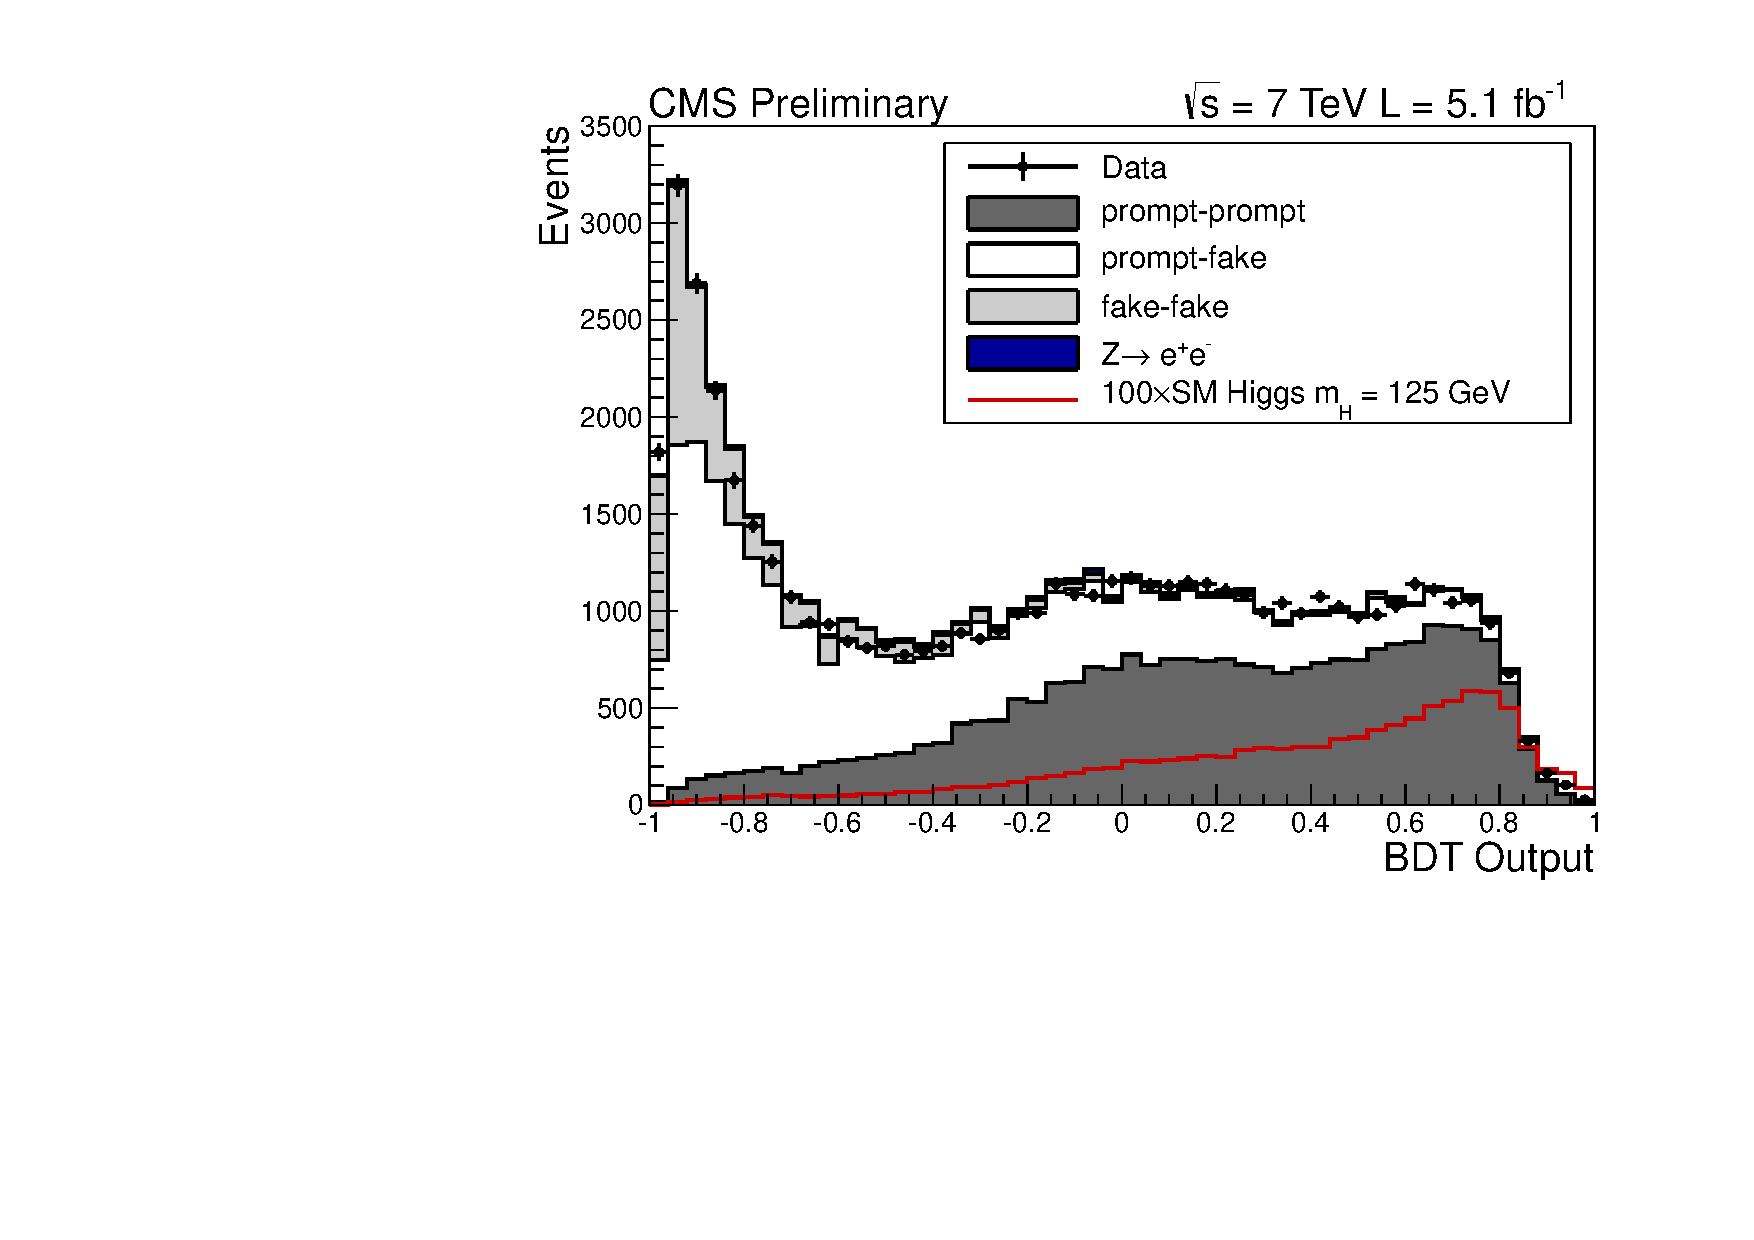
\includegraphics[width=0.8\textwidth]{hgg7TeV/variablePlots/bdtoutput_full}
 \caption{Diphoton BDT distribution in data and MC. The contribution expected from a SM Higgs with mass 125 GeV, 
 scaled by 100, is shown in red. }
 \label{fig:diphotonBDT}
\end{center}
\end{figure}

Figures~\ref{fig:diphotonbdtvars1} and~\ref{fig:diphotonbdtvars2} show the input variables from the 
final set of selected diphoton candidates in data and MC. 
The expectation in each plot from a SM Higgs with a mass of 125 GeV, scaled by 10, is shown in red. 
The invariant mass distribution in data and MC for events passing the full
selection is given in Figure~\ref{fig:massmcdata}. After the application of the full selection, 
the total background contains around 76\% prompt diphoton events.

\begin{figure}[hbt!]
\begin{center}
  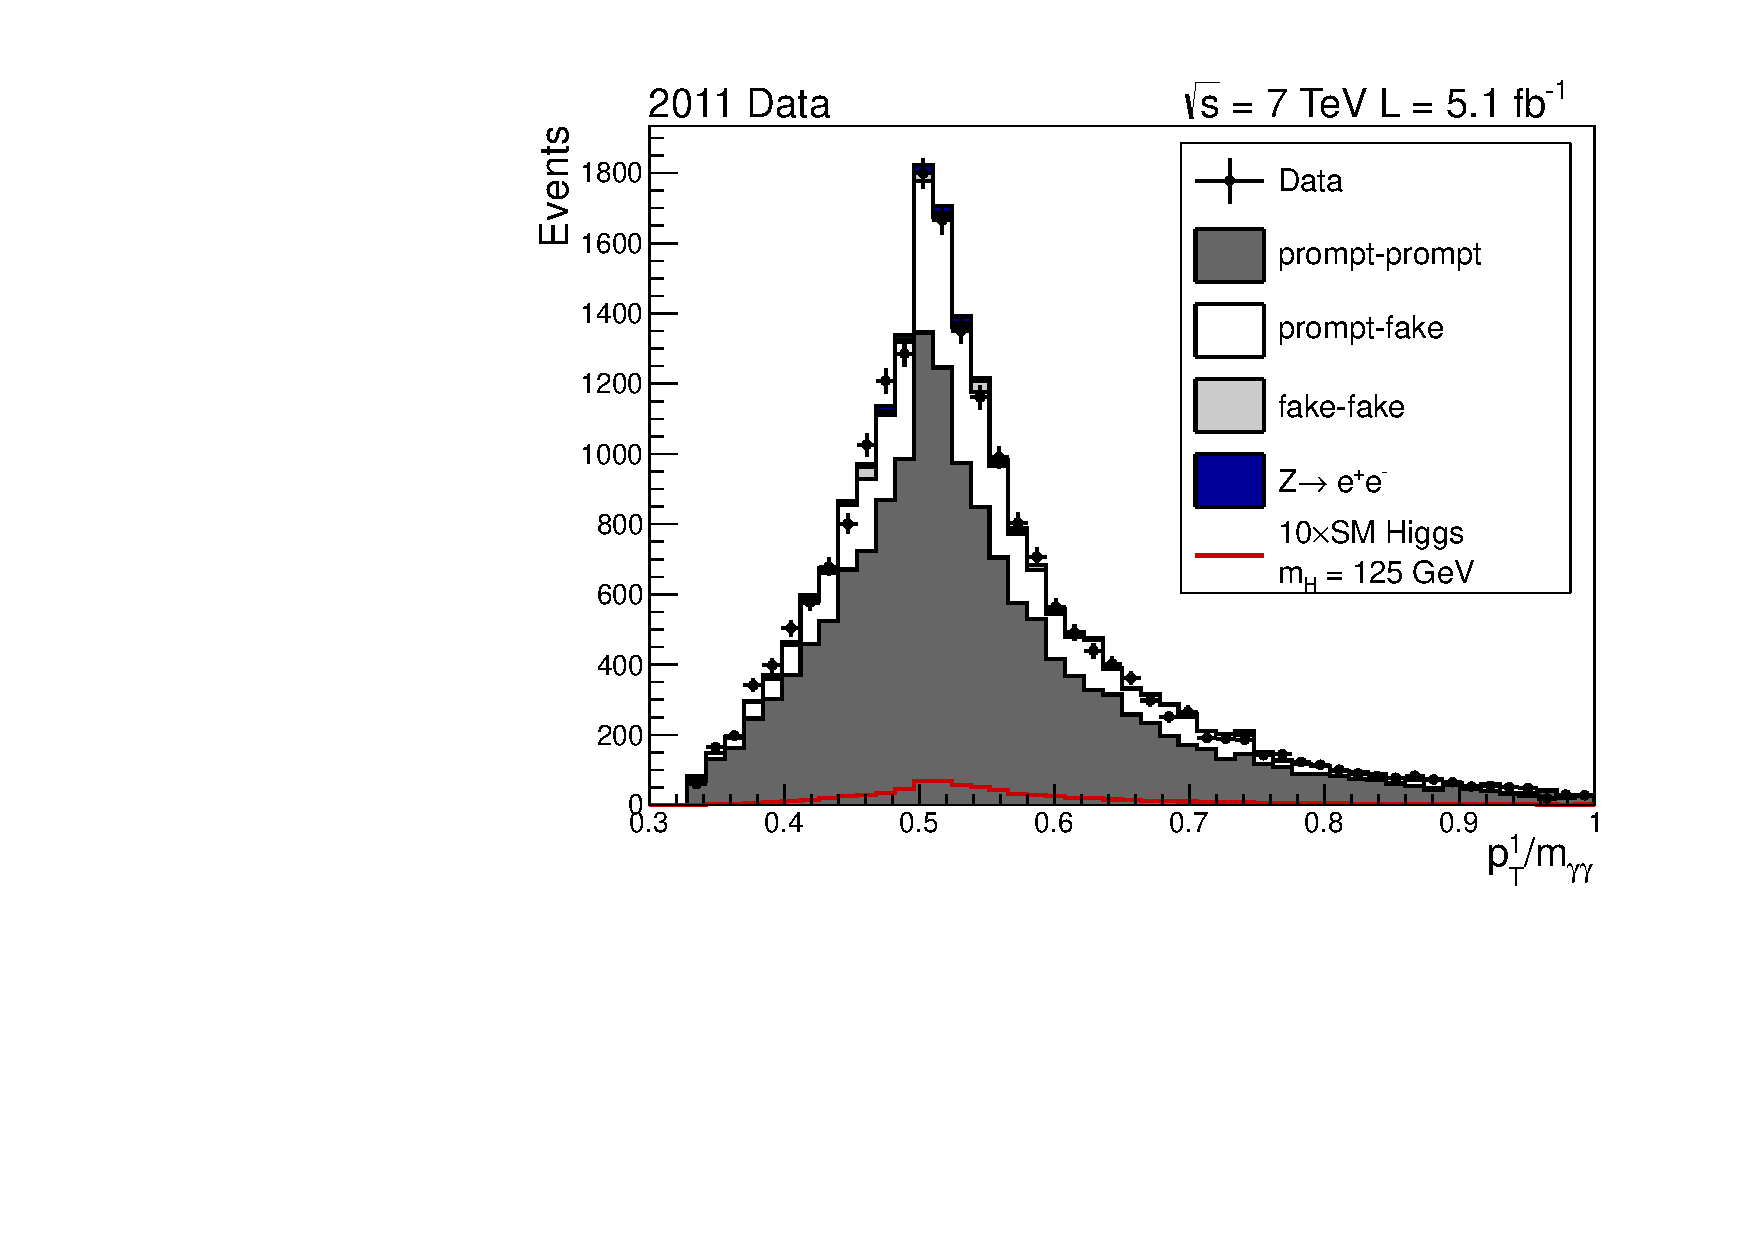
\includegraphics[width=0.48\textwidth]{hgg7TeV/variablePlots/pt_1om}
  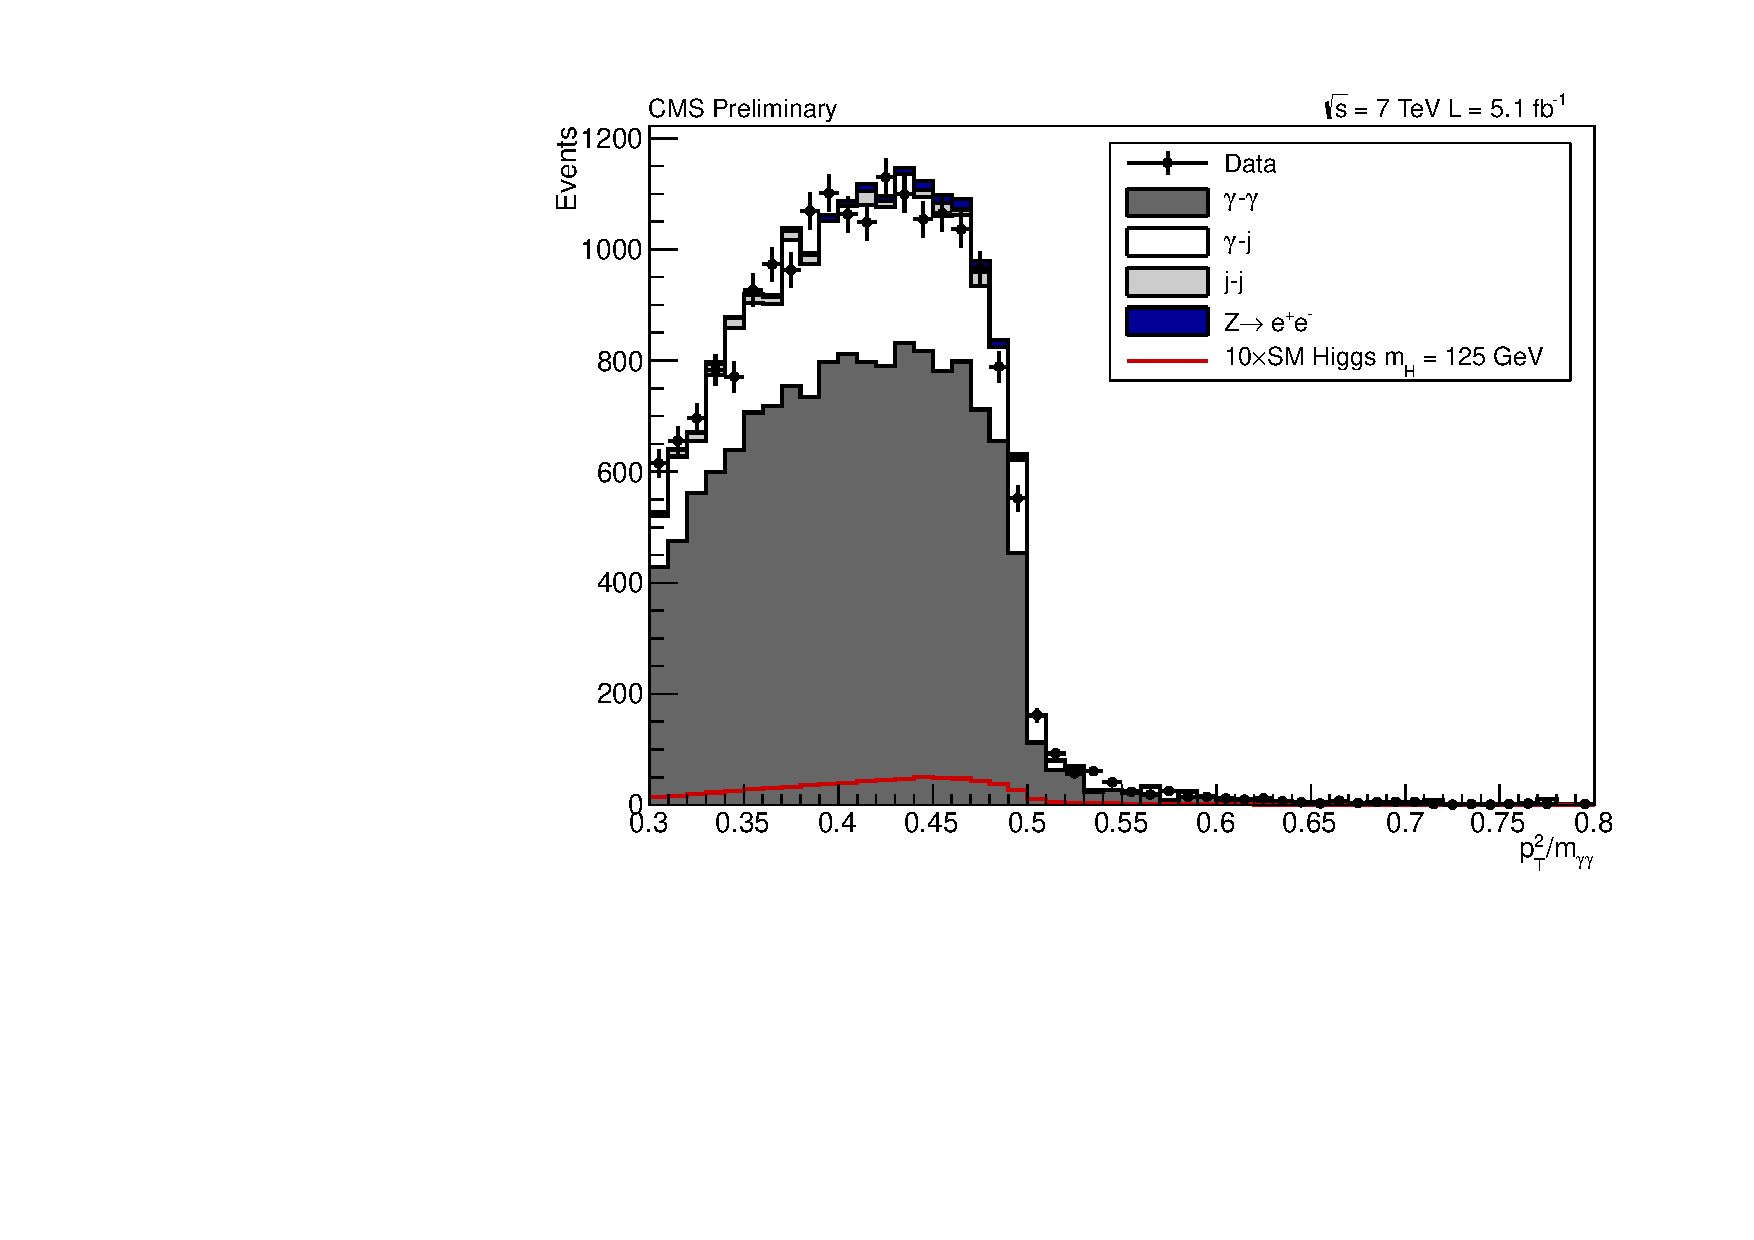
\includegraphics[width=0.48\textwidth]{hgg7TeV/variablePlots/pt_2om}\\
  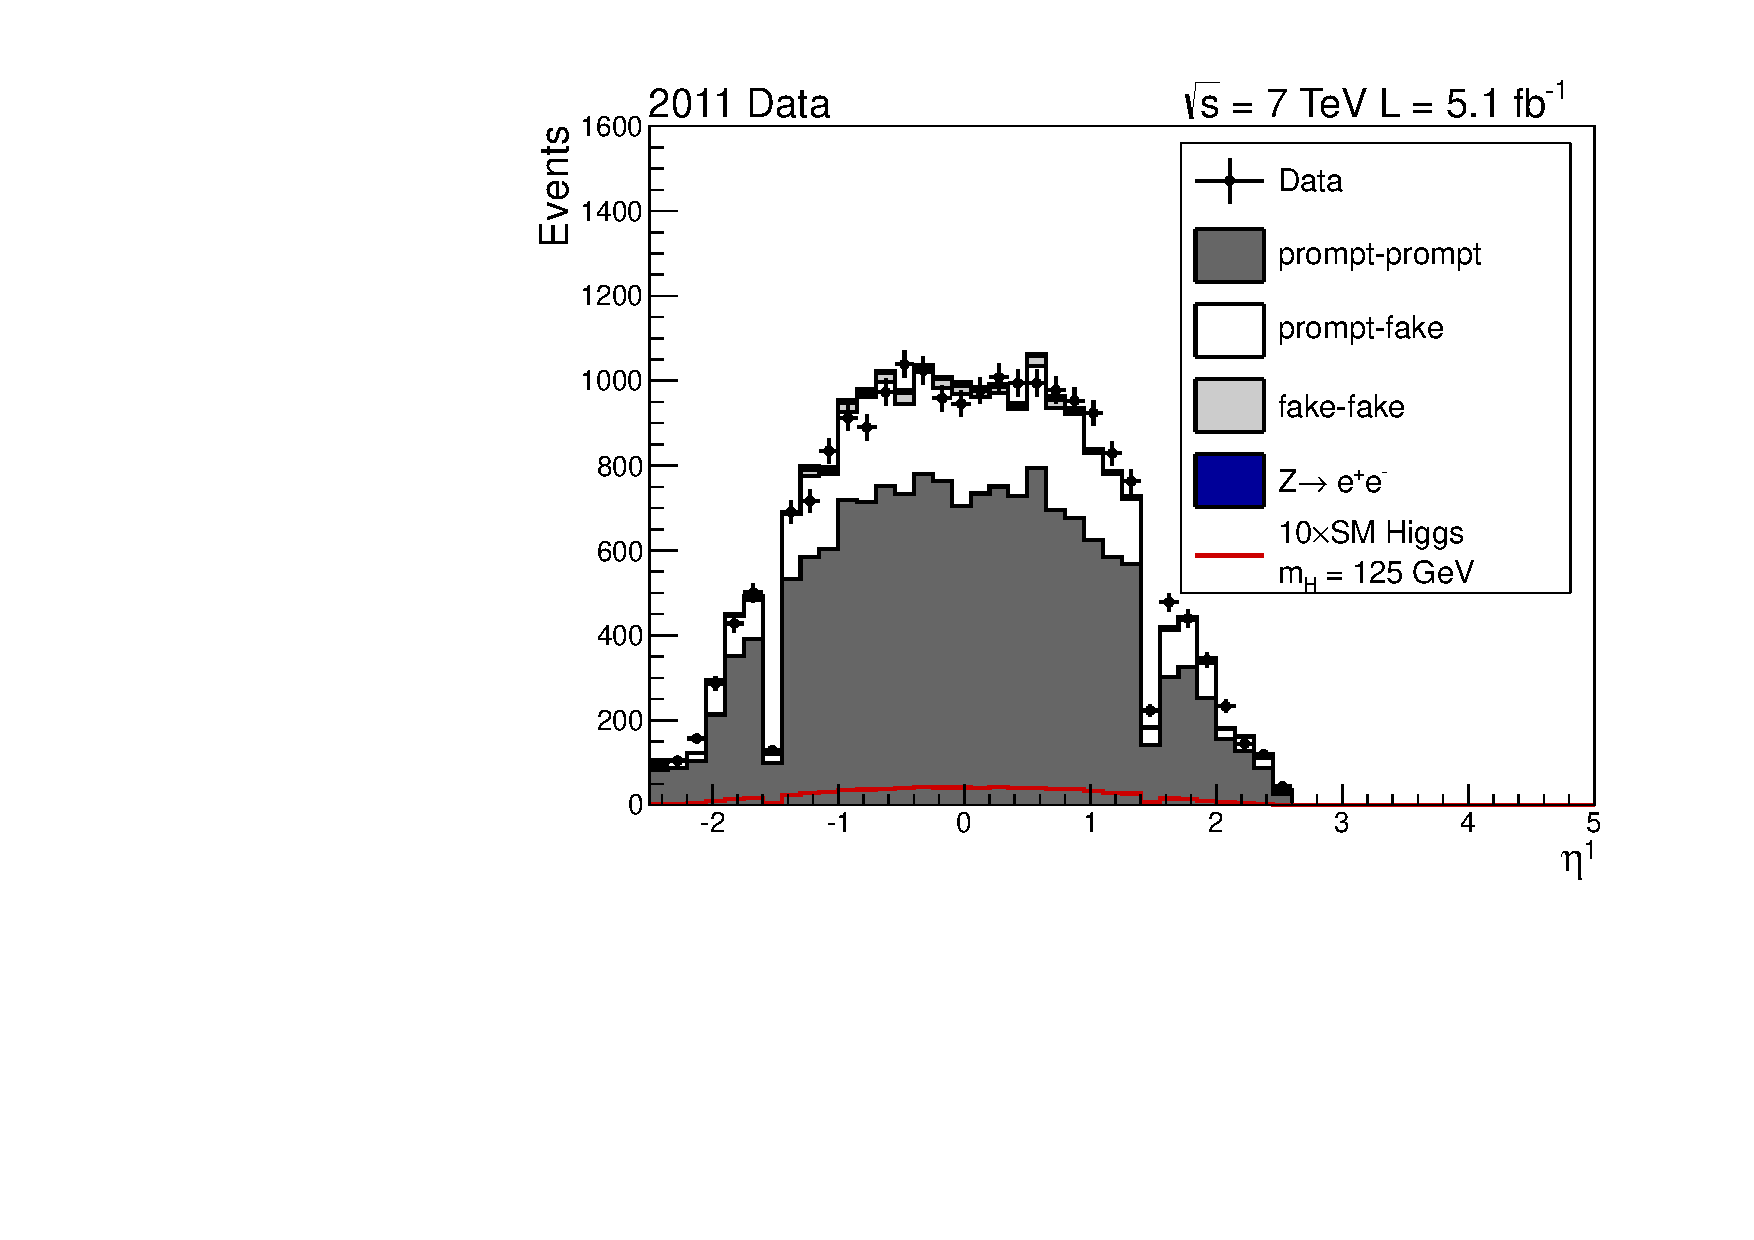
\includegraphics[width=0.48\textwidth]{hgg7TeV/variablePlots/phoeta_1}
  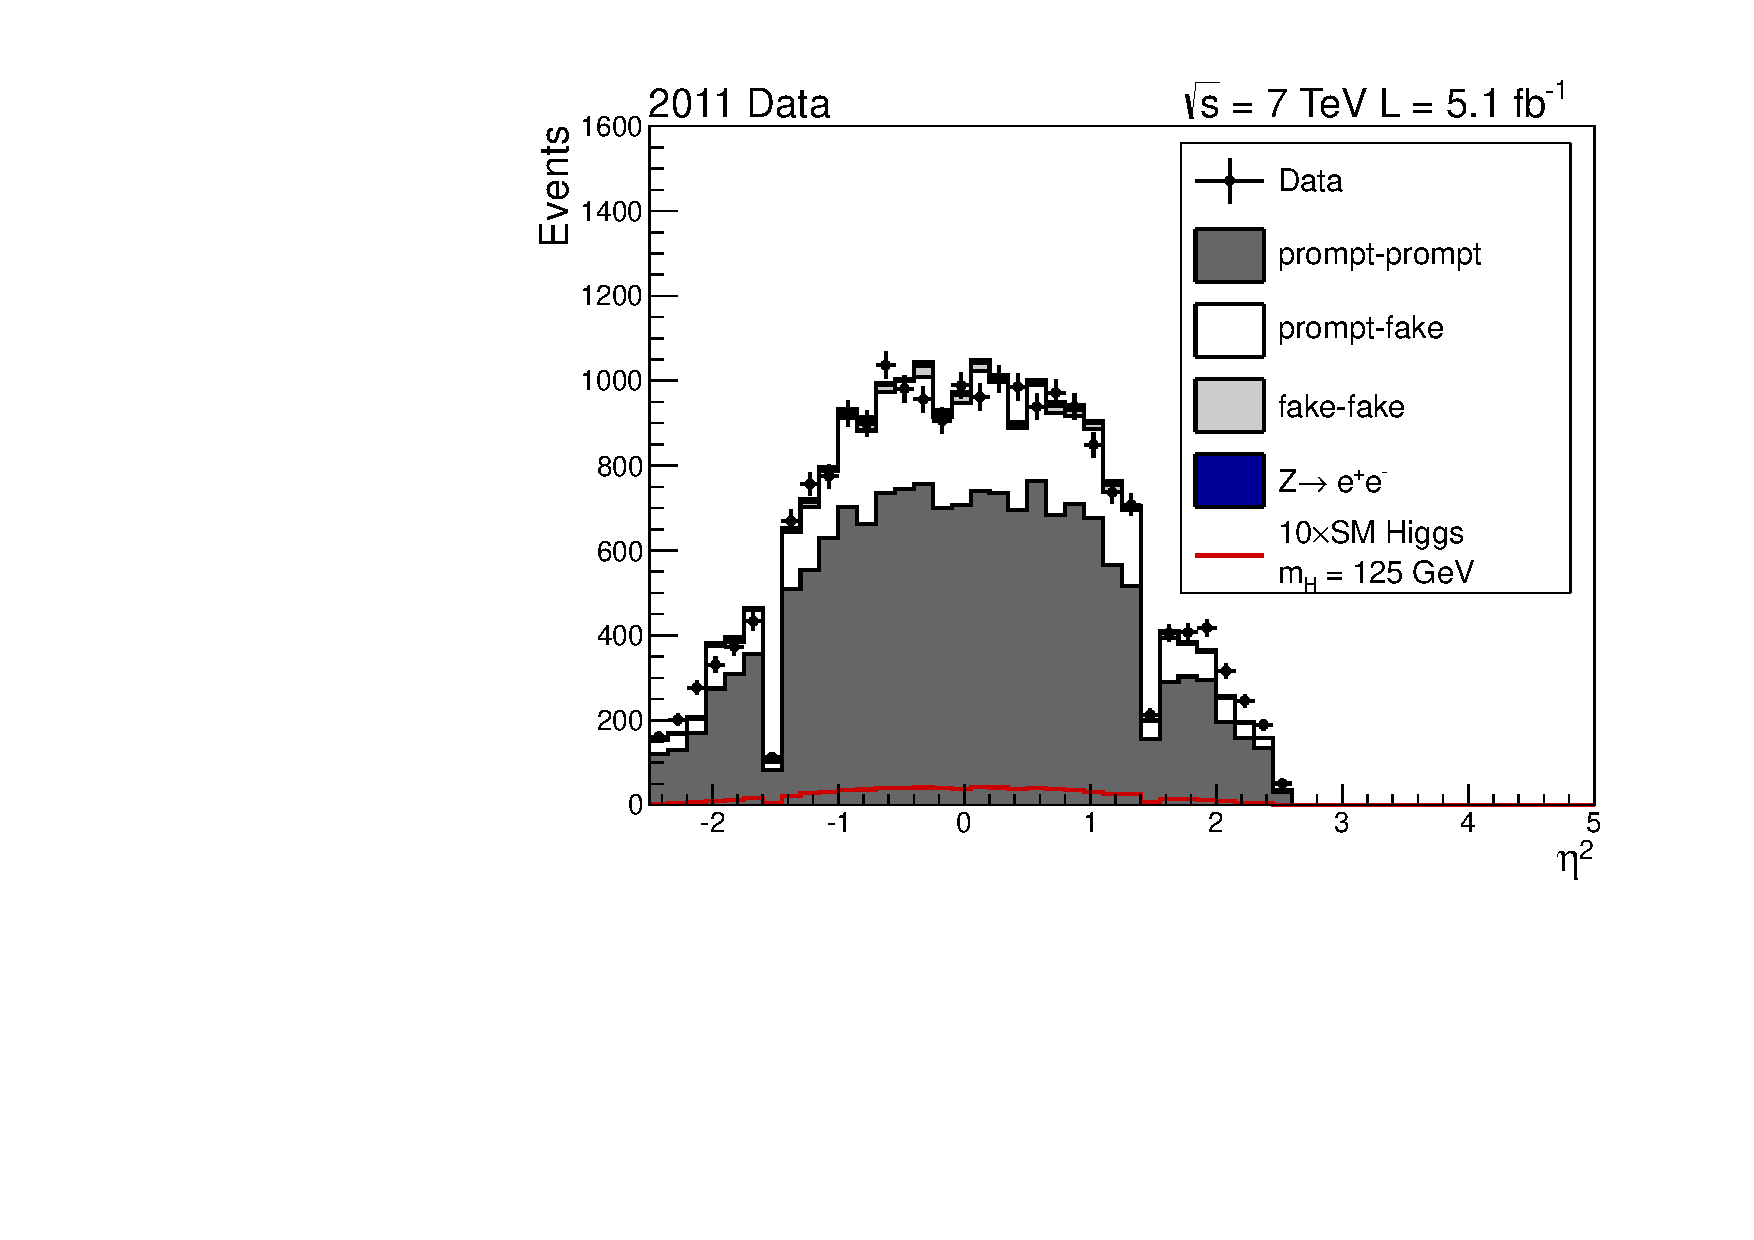
\includegraphics[width=0.48\textwidth]{hgg7TeV/variablePlots/phoeta_2}\\
  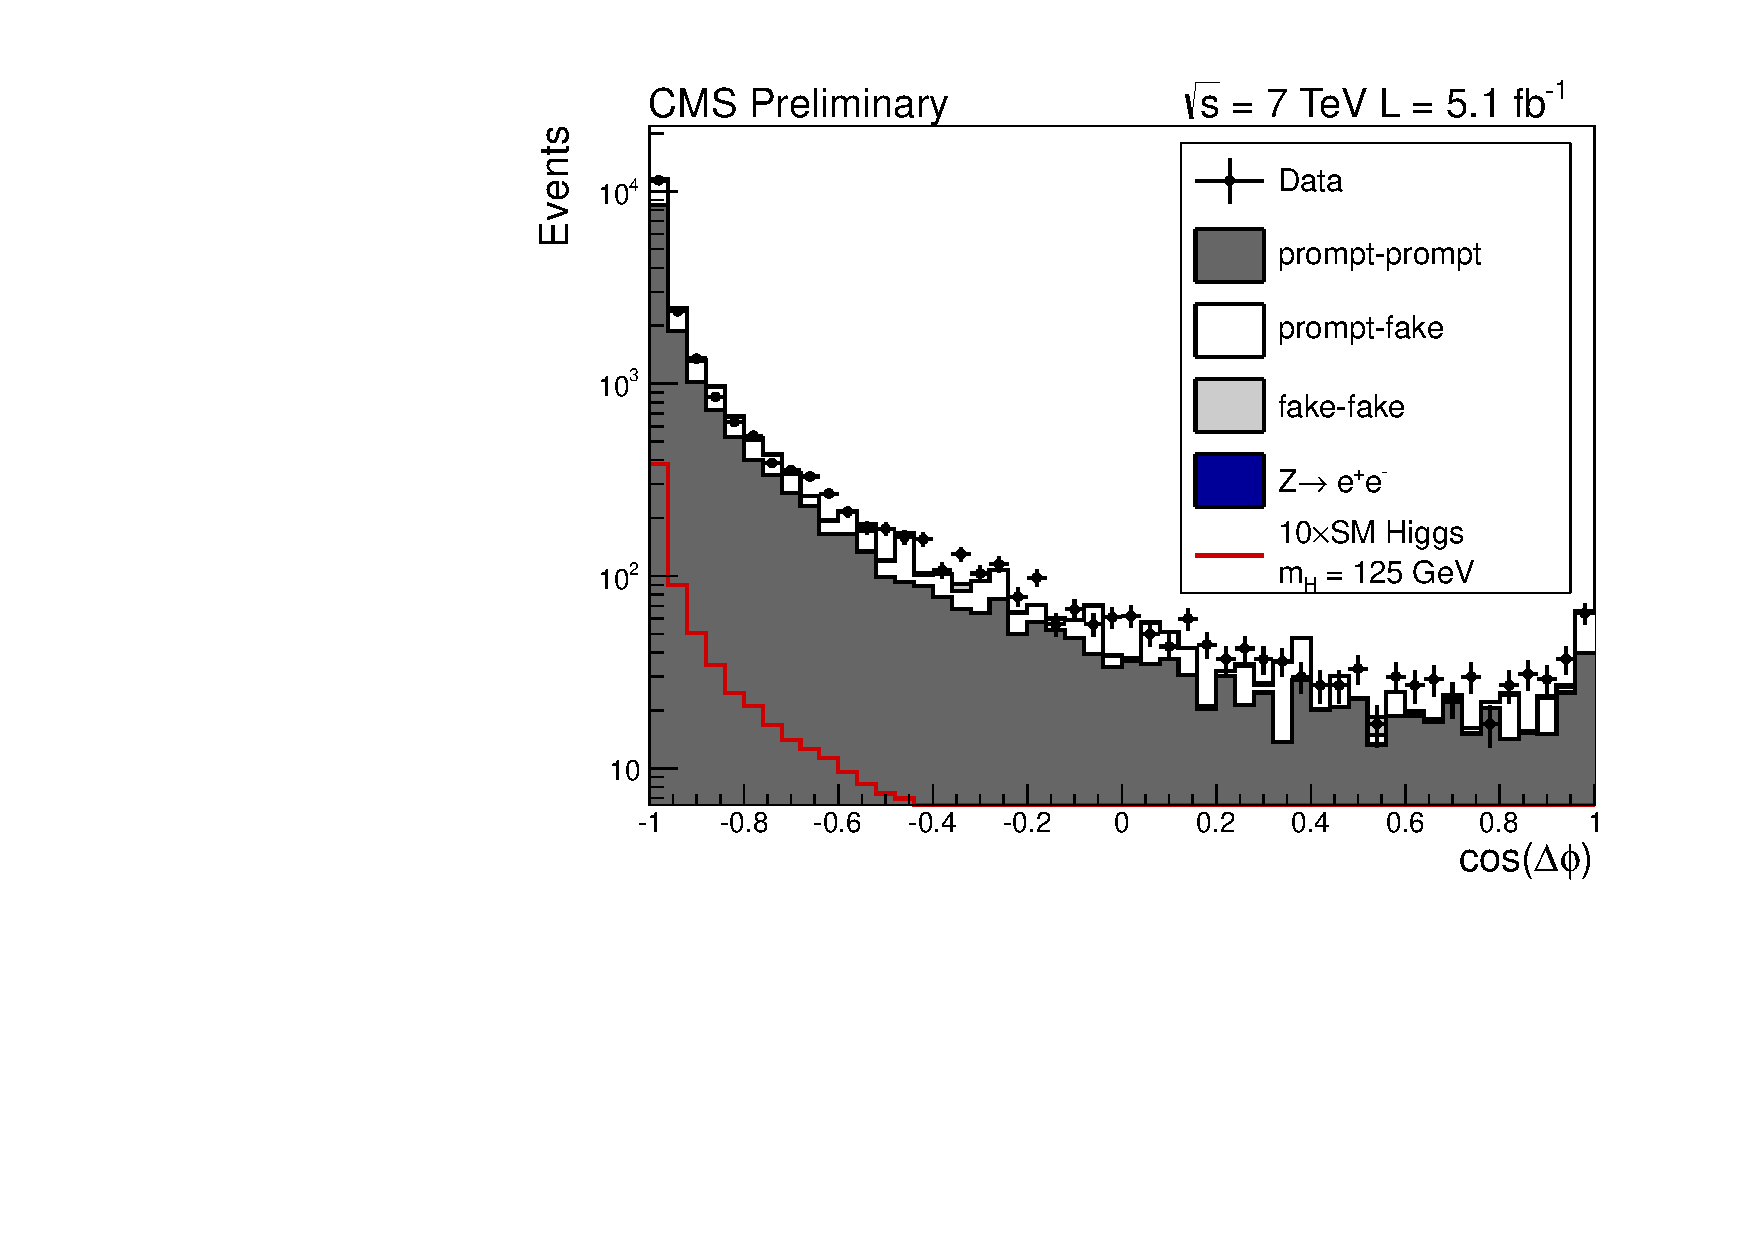
\includegraphics[width=0.48\textwidth]{hgg7TeV/variablePlots/cosdphi}
 \label{fig:diphotonbdtvars1}
 \caption{Kinematic diphoton BDT input variable distributions in data and MC. 
	  The distributions are for events which pass the full selection 
	  including a cut on the diphoton BDT output of 0.05.
 	  The expectation from a SM Higgs with 125 GeV is shown in red.}
\end{center}
\end{figure}

\begin{figure}[hbt!]
\begin{center}
  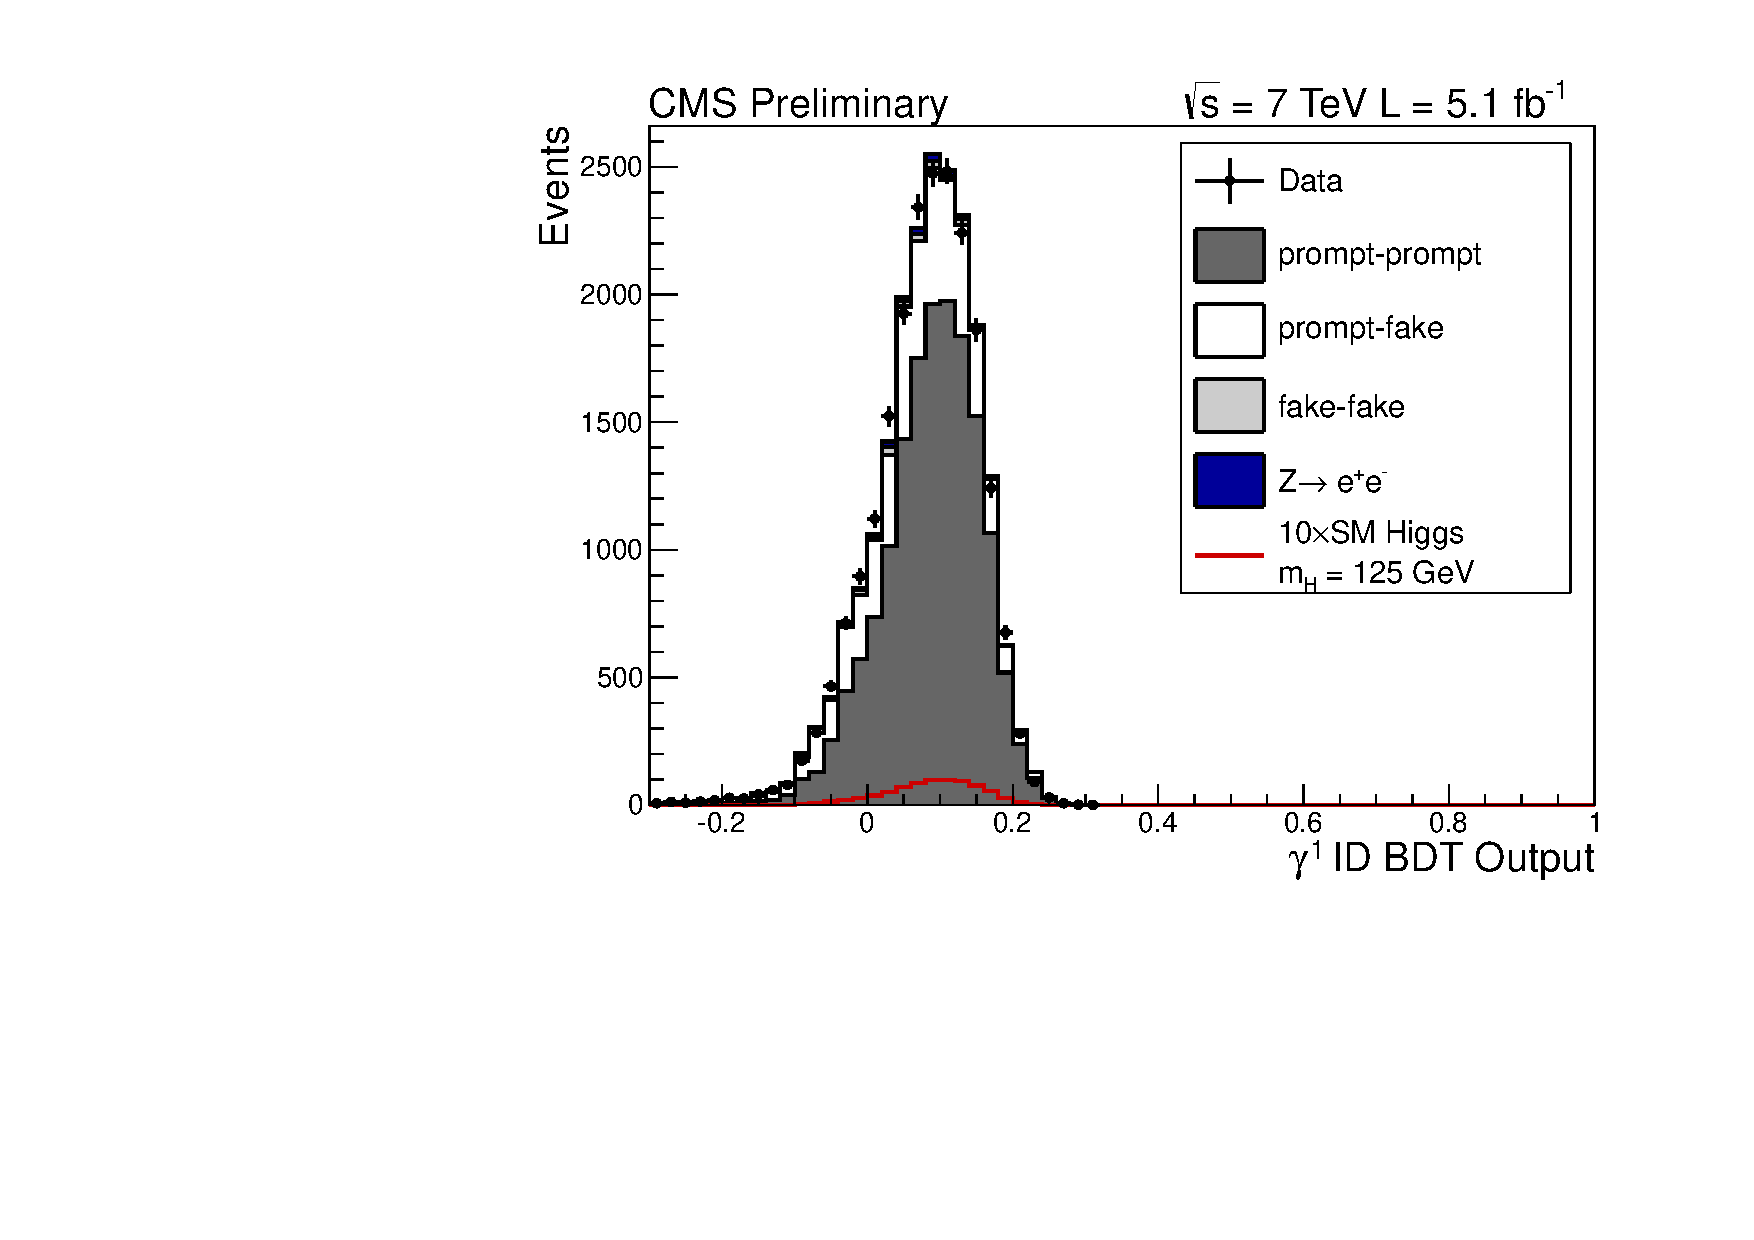
\includegraphics[width=0.48\textwidth]{hgg7TeV/variablePlots/phoid_1}
  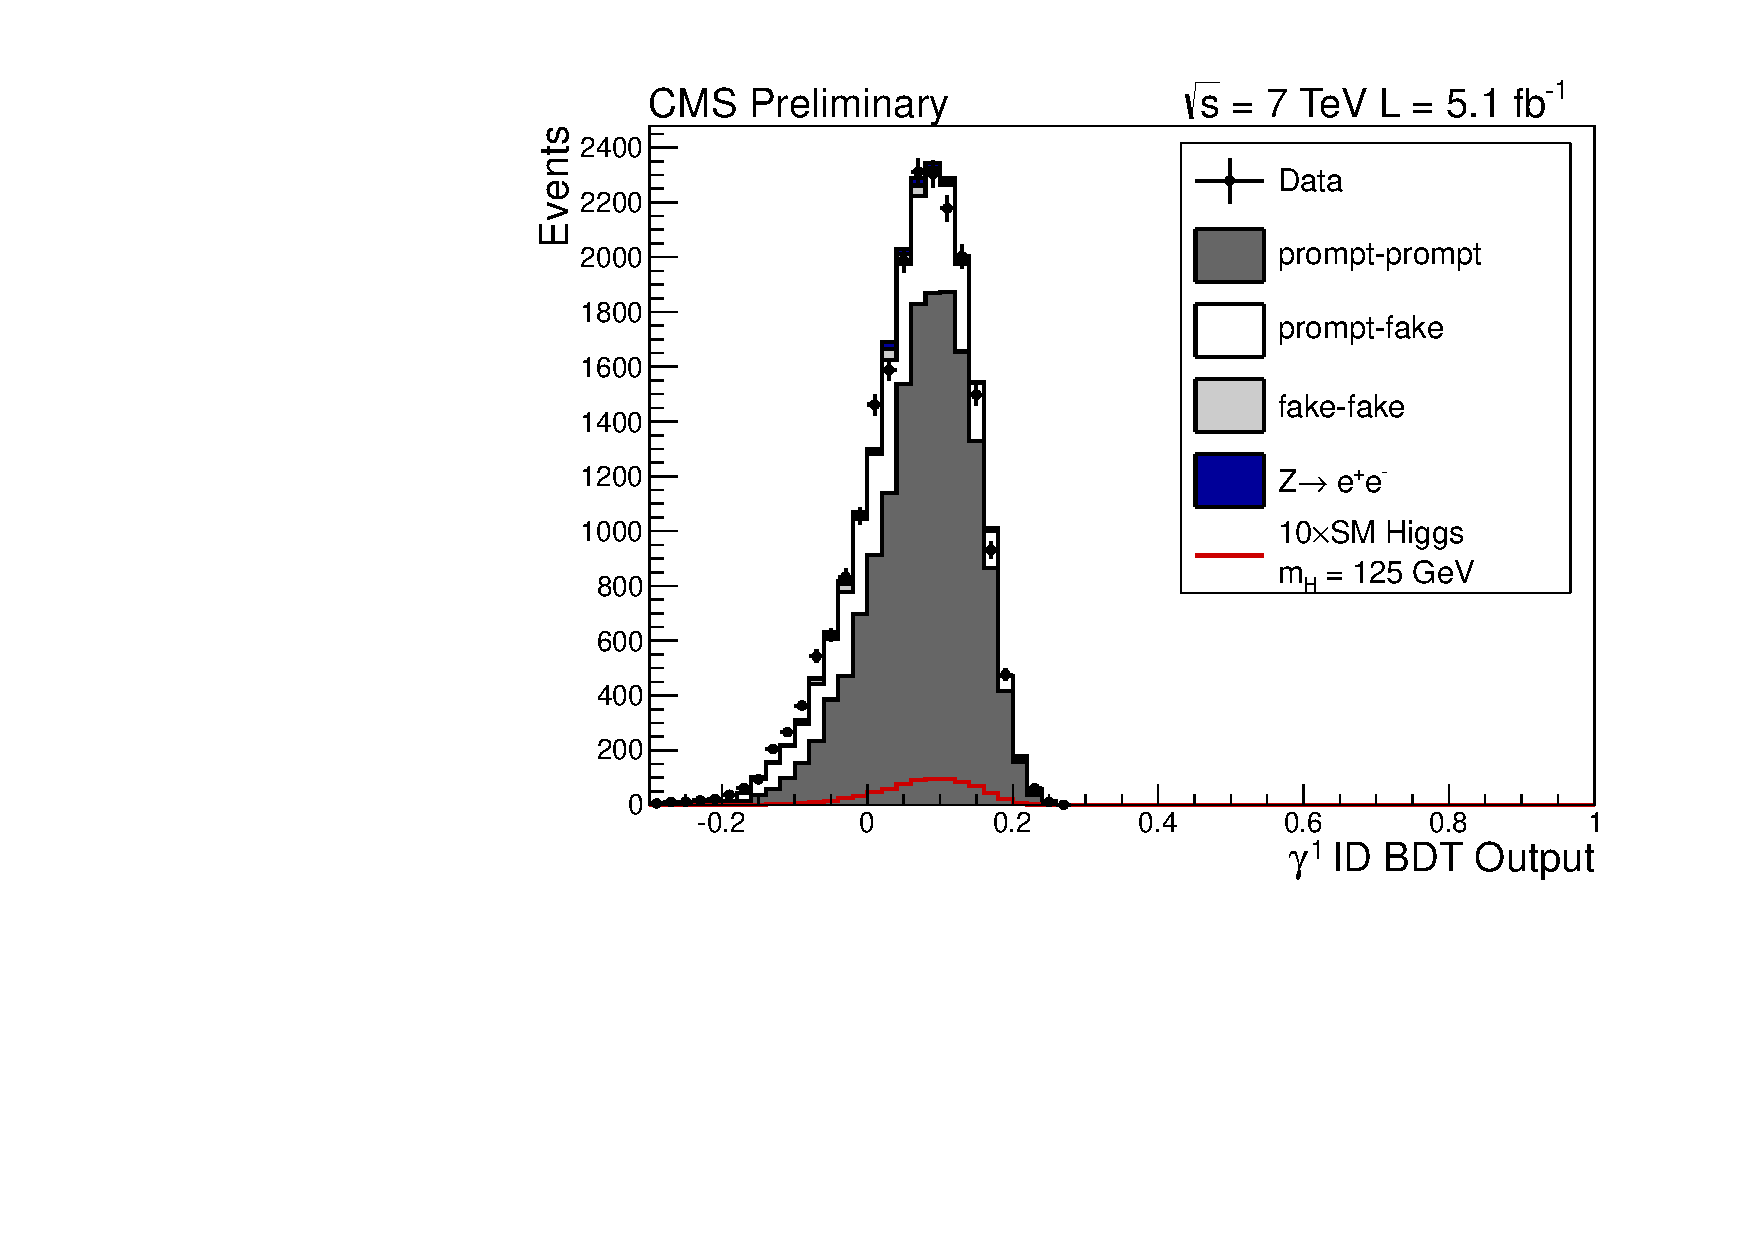
\includegraphics[width=0.48\textwidth]{hgg7TeV/variablePlots/phoid_2}\\
  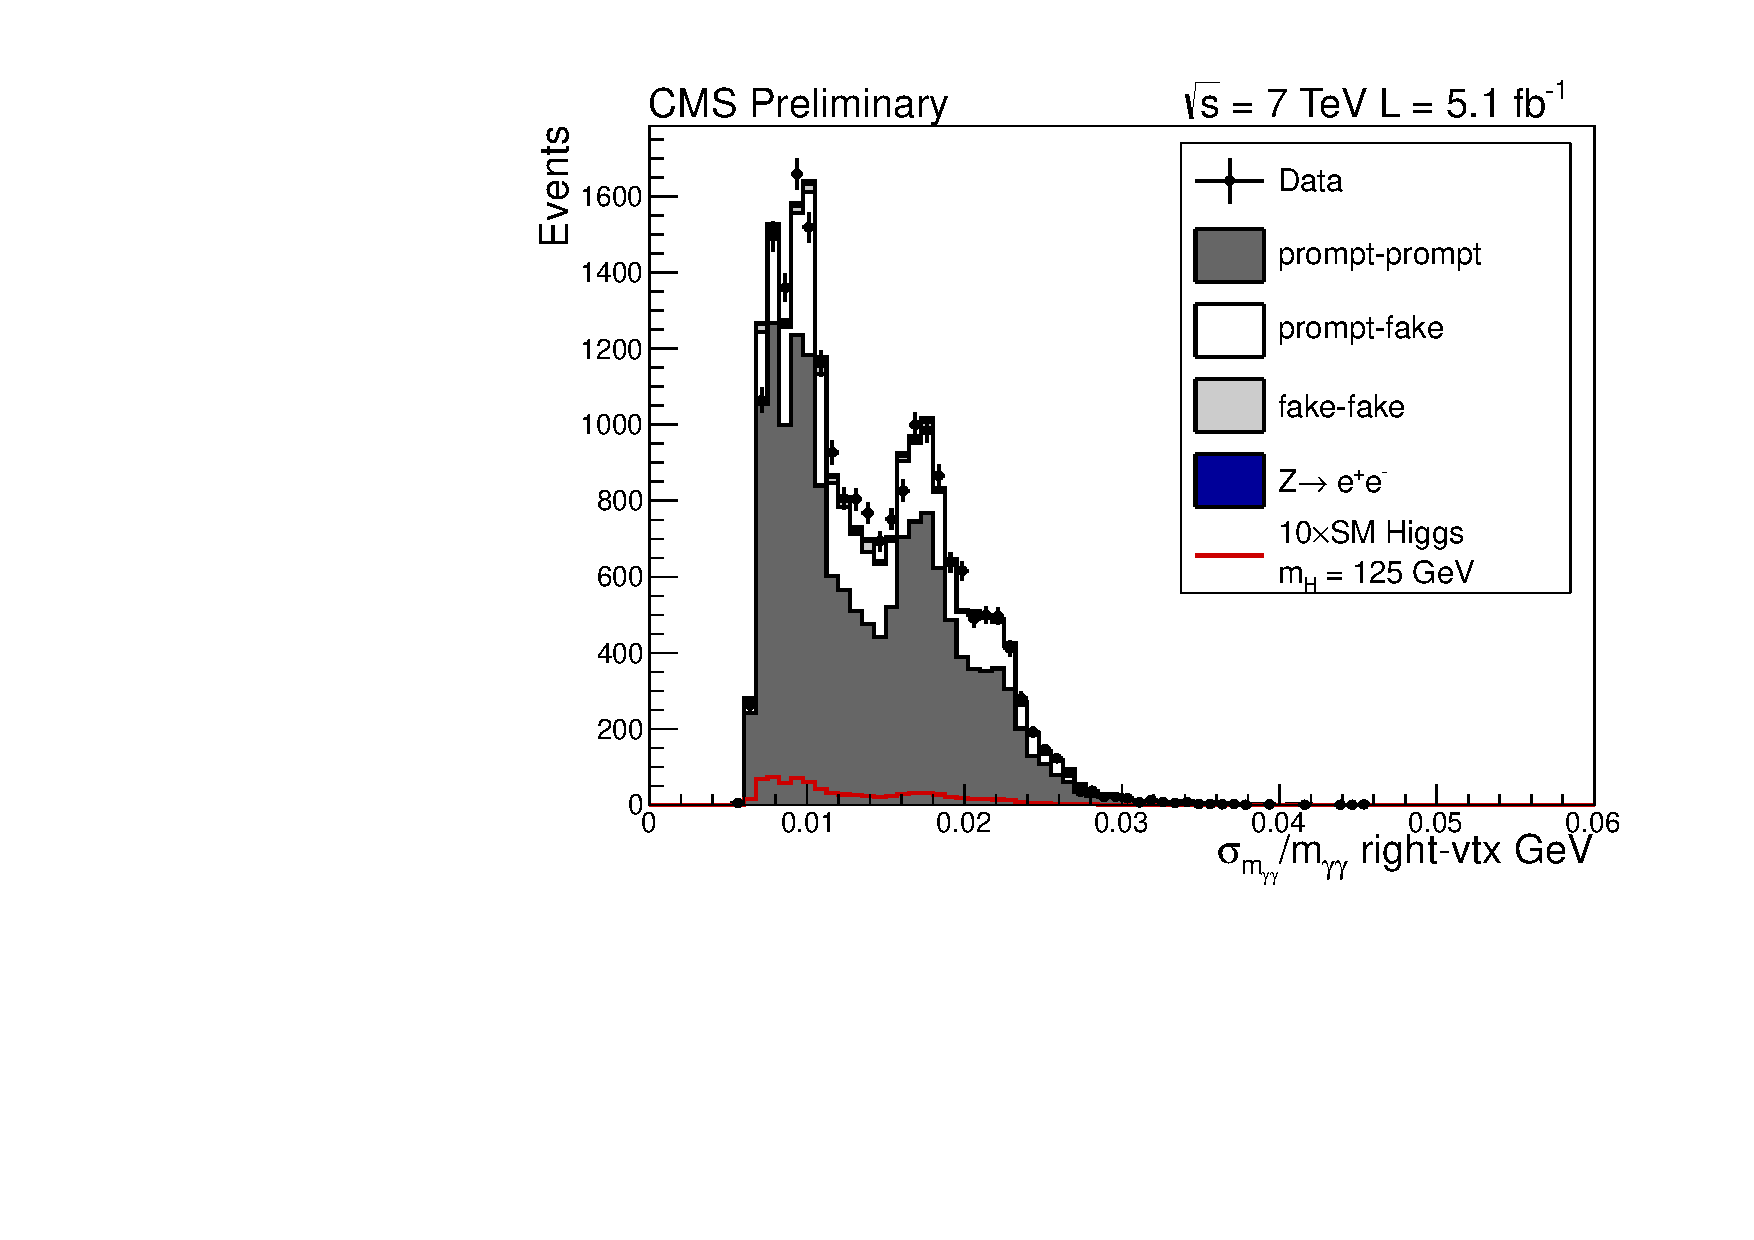
\includegraphics[width=0.48\textwidth]{hgg7TeV/variablePlots/sigmrv}
  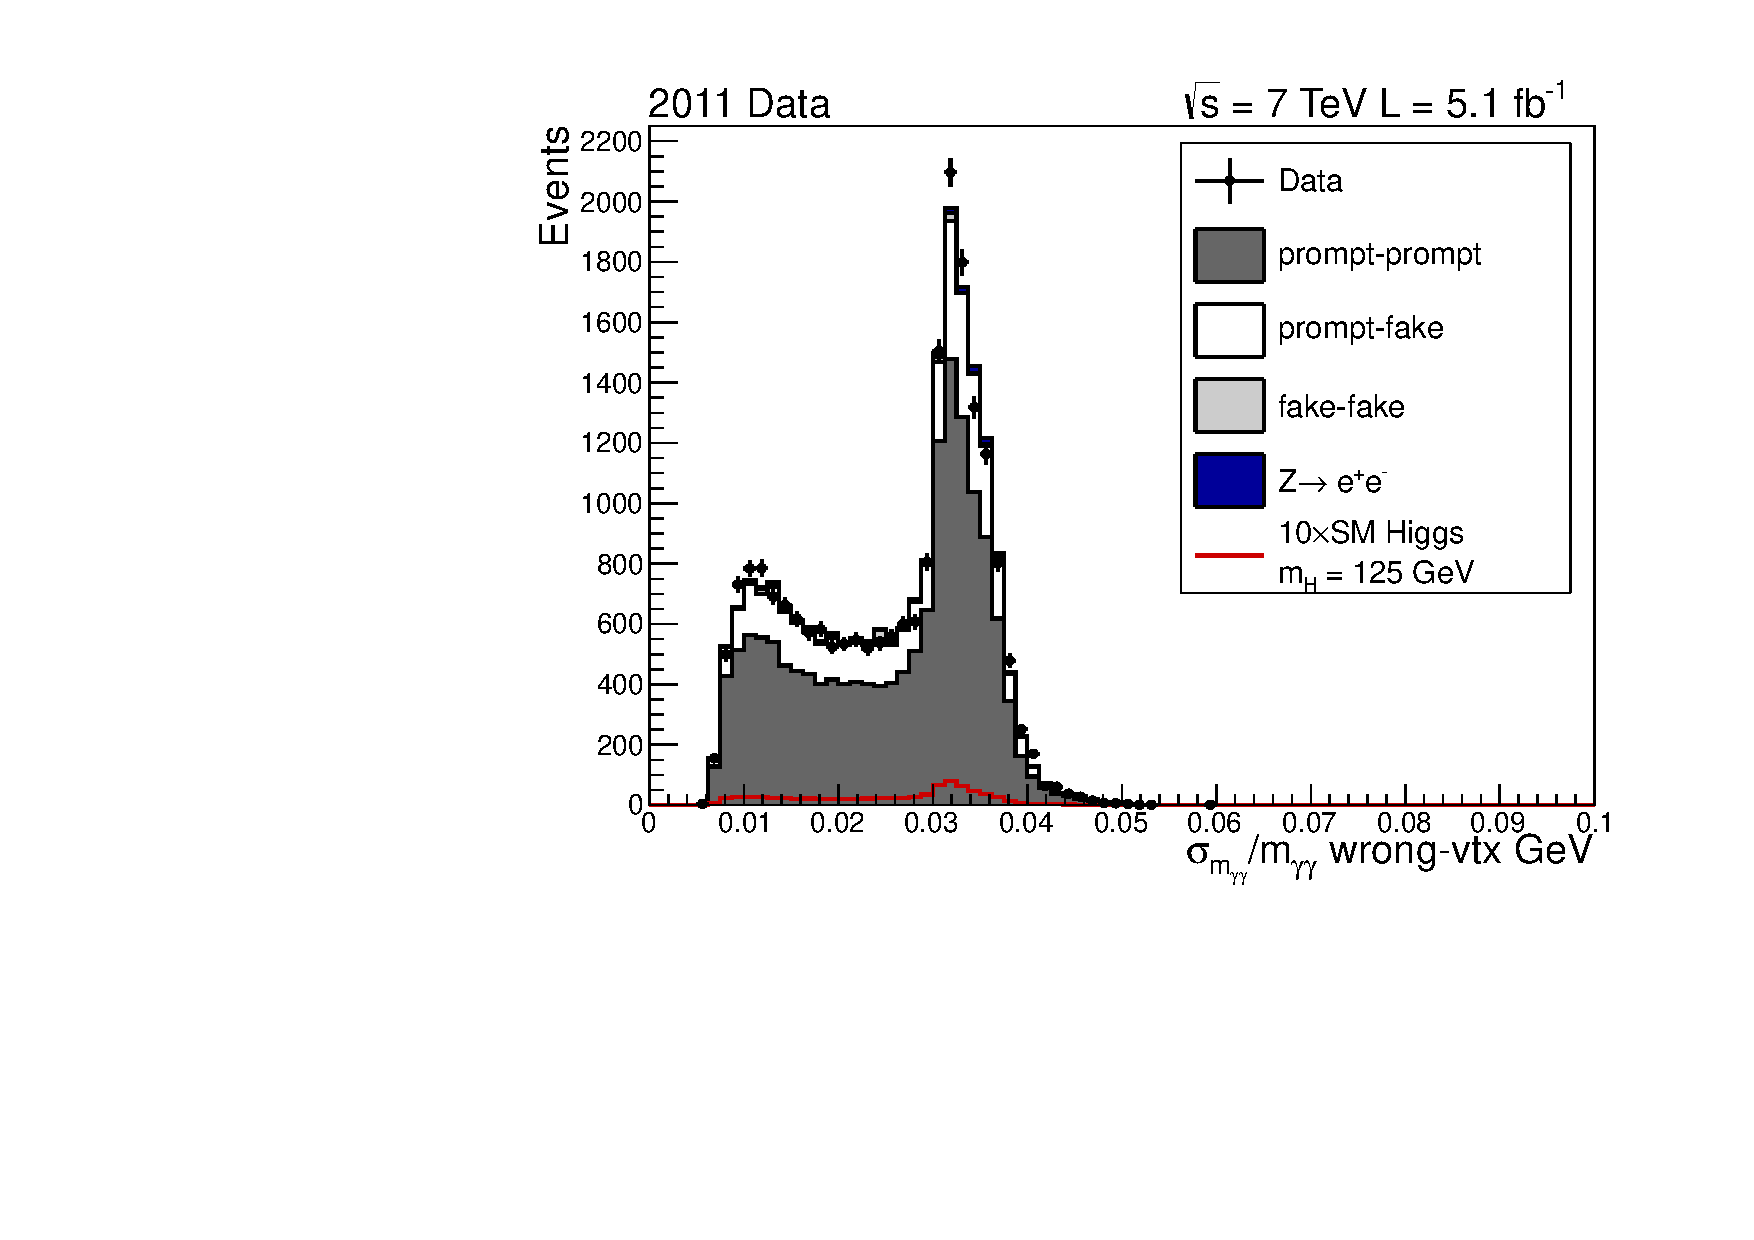
\includegraphics[width=0.48\textwidth]{hgg7TeV/variablePlots/sigmwv}
 \label{fig:diphotonbdtvars2}
 \caption{Additional diphoton BDT input variable distributions in data and MC. 
	  The distributions are for events which pass the full selection 
	  including a cut on the diphoton BDT output of 0.05.
 	  The expectation from a SM Higgs with 125 GeV is shown in red.}
\end{center}
\end{figure}

\begin{figure}[hbt!]
\begin{center}
  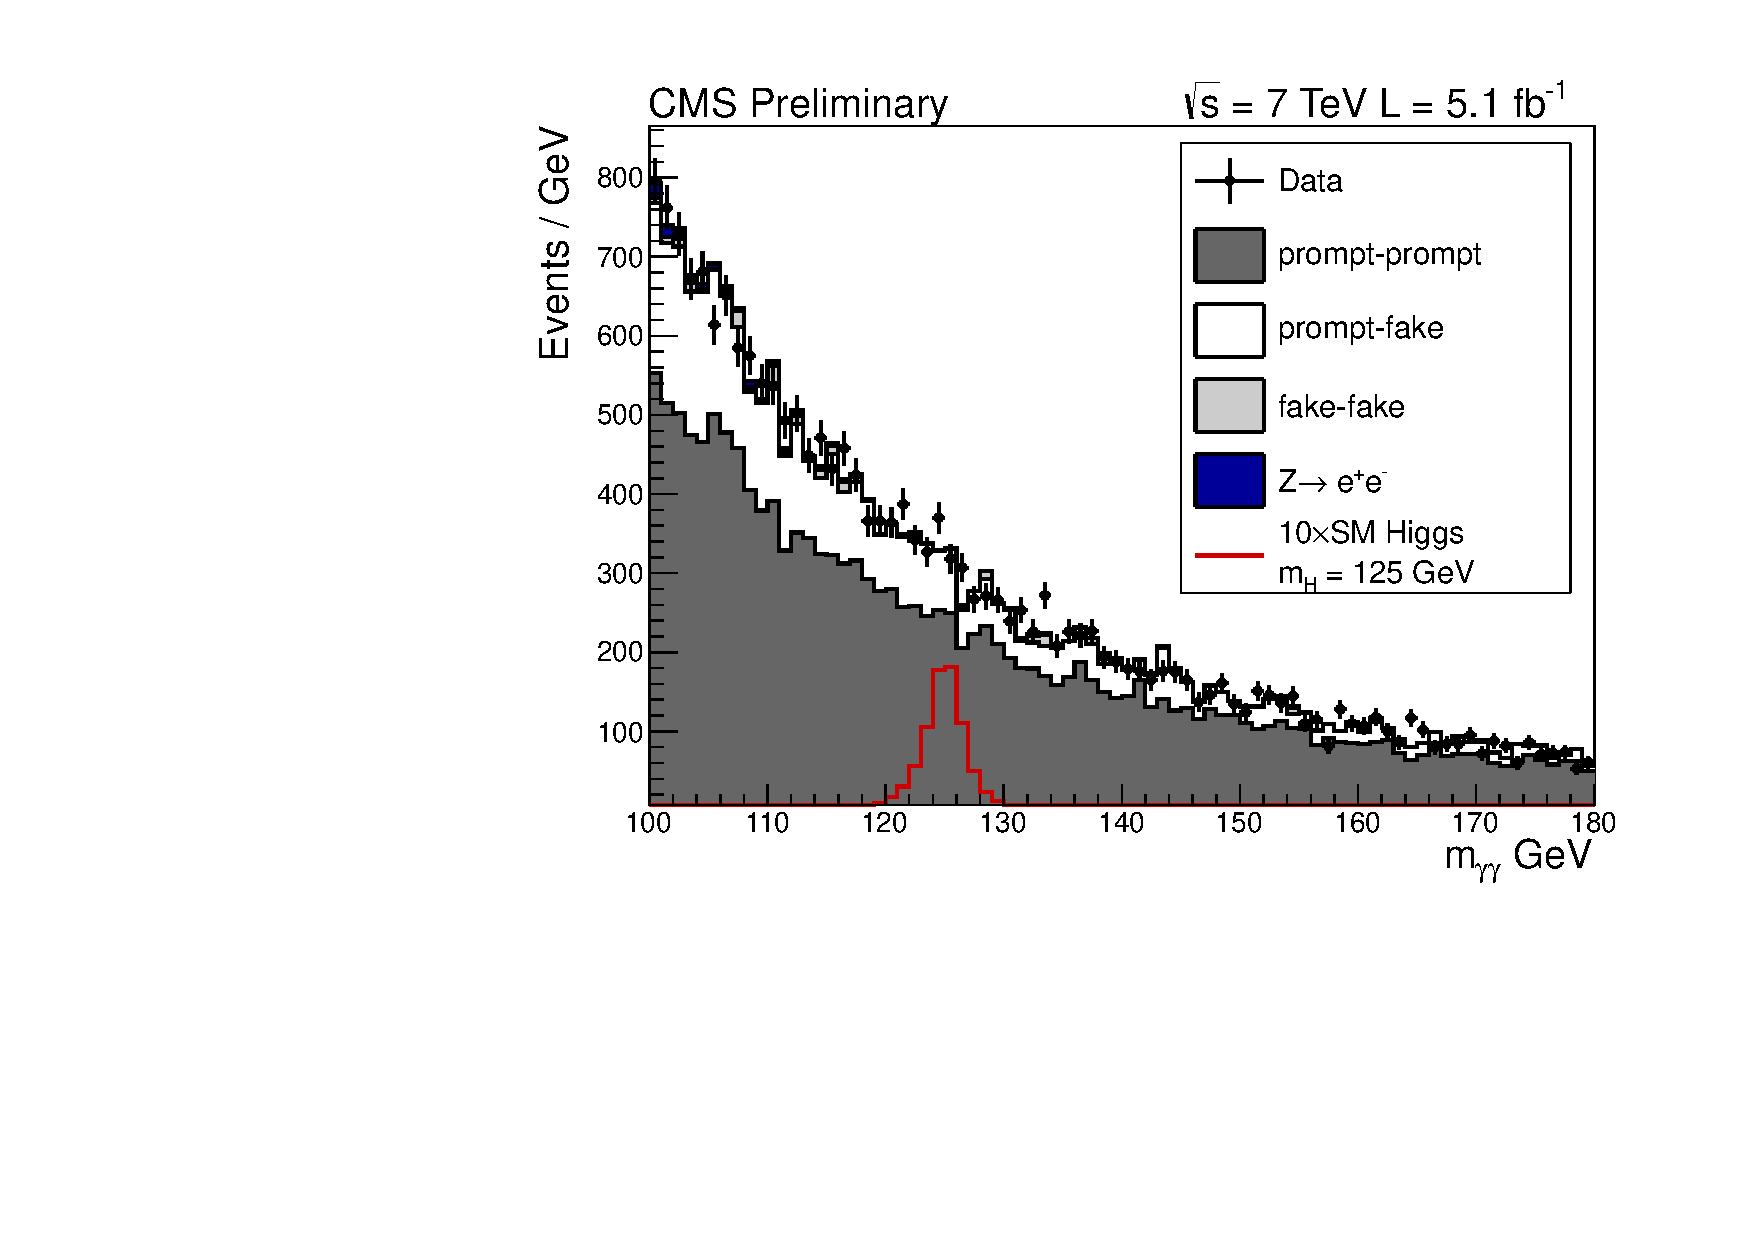
\includegraphics[width=0.8\textwidth]{hgg7TeV/variablePlots/mass}
 \caption{Invariant mass distrobution in data and MC after applying the full event selection in the
 range 100 to 180 GeV. The contribution expected from a SM Higgs with mass 125 GeV, scaled by 10, 
 is shown in red. }
 \label{fig:massmcdata}
\end{center}
\end{figure}

\subsubsection{Diphoton BDT Validation with $\Zee$ Data}
By using a BDT for the full event selection, subtle correlations between the input variables are acounted for
which improves the separation between the signal and background. 
Unlike the background model, the signal model will be taken from corrected MC simulation. 
It is important therefore to ensure that the BDT will respond in the same way in data as for the signal MC
used for the signal extraction. The MC can be validated using $\Zee$ data-MC
comparisons by inverting the electron veto and treating the electrons as though they were photons.
This is done by using the supercluster associated to the electron for the electron's energy measurement 
and ignoring the track information. In this way, the reconstruction of the electrons is the same as that
of the photons allowing for validation of the BDT's response to real photons from a resonance decay~\cite{null}. 
Figure~\ref{fig:zeevaliddiphomva} shows the diphoton BDT distribution in $\Zee$ MC and data after applying
the full selection using this technique. 

\begin{figure}
\begin{center}
  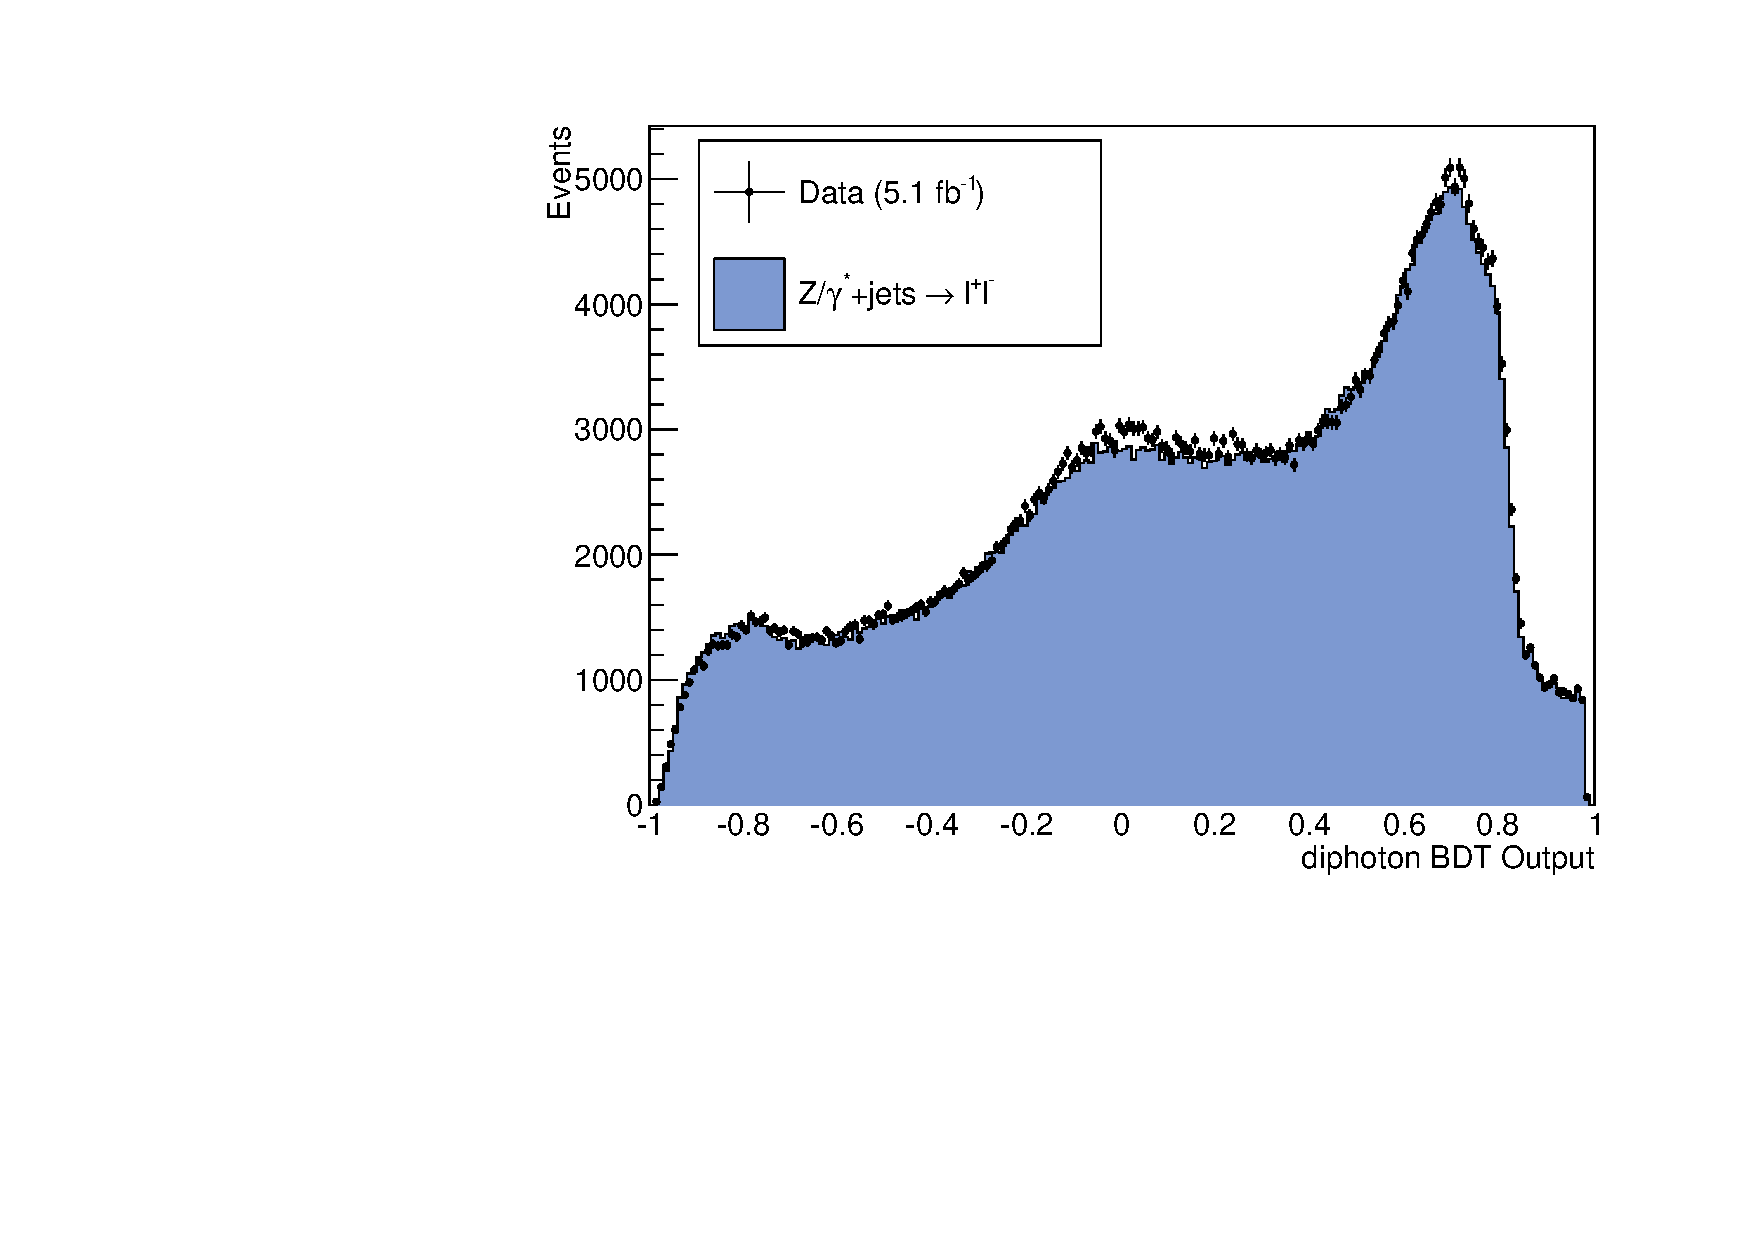
\includegraphics[width=.6\textwidth]{hgg7TeV/zeeValidation/zeevalidationdipho.pdf}
\label{fig:zeevaliddiphomva}
\caption{Diphoton BDT output distribution in $\Zee$ MC and data after the full selection 
treating the electrons as photons for the purposes of energy reconstruction. The electron 
veto is inverted to preferentially select electrons.}
\end{center}
\end{figure}

Both the photon ID and regression BDT rely on a detailed simulation of electromagnetic showering  
in MC to correctly describe the data. Due to impoerfections of this simulation, systematic
uncertainties are included in the signal model to cover the residual difference observed between MC and data
in a high $\pt$ photons. 
These uncertainties are validated using $\Zee$ in the same way as the diphoton BDT. 
Figures~\ref{fig:zeevalidsigmaE} and~\ref{fig:zeevailidphoidmva} show the distributions of the 
per photon energy resolution estimator $\sigma_{E}$ relative to the photon energy and the output of the 
photon ID BDT in $\Zee$ MC and data treating the electrons as photons. The red lines
show the $\pm 1\sigma$ error envelope attributed to the systematic uncertainty on the shower simulation.
These uncertainties are propagated through the diphoton BDT and included in the signal model as described in 
Section~\ref{sec:signalmodel}.

\begin{figure}
\begin{center}
  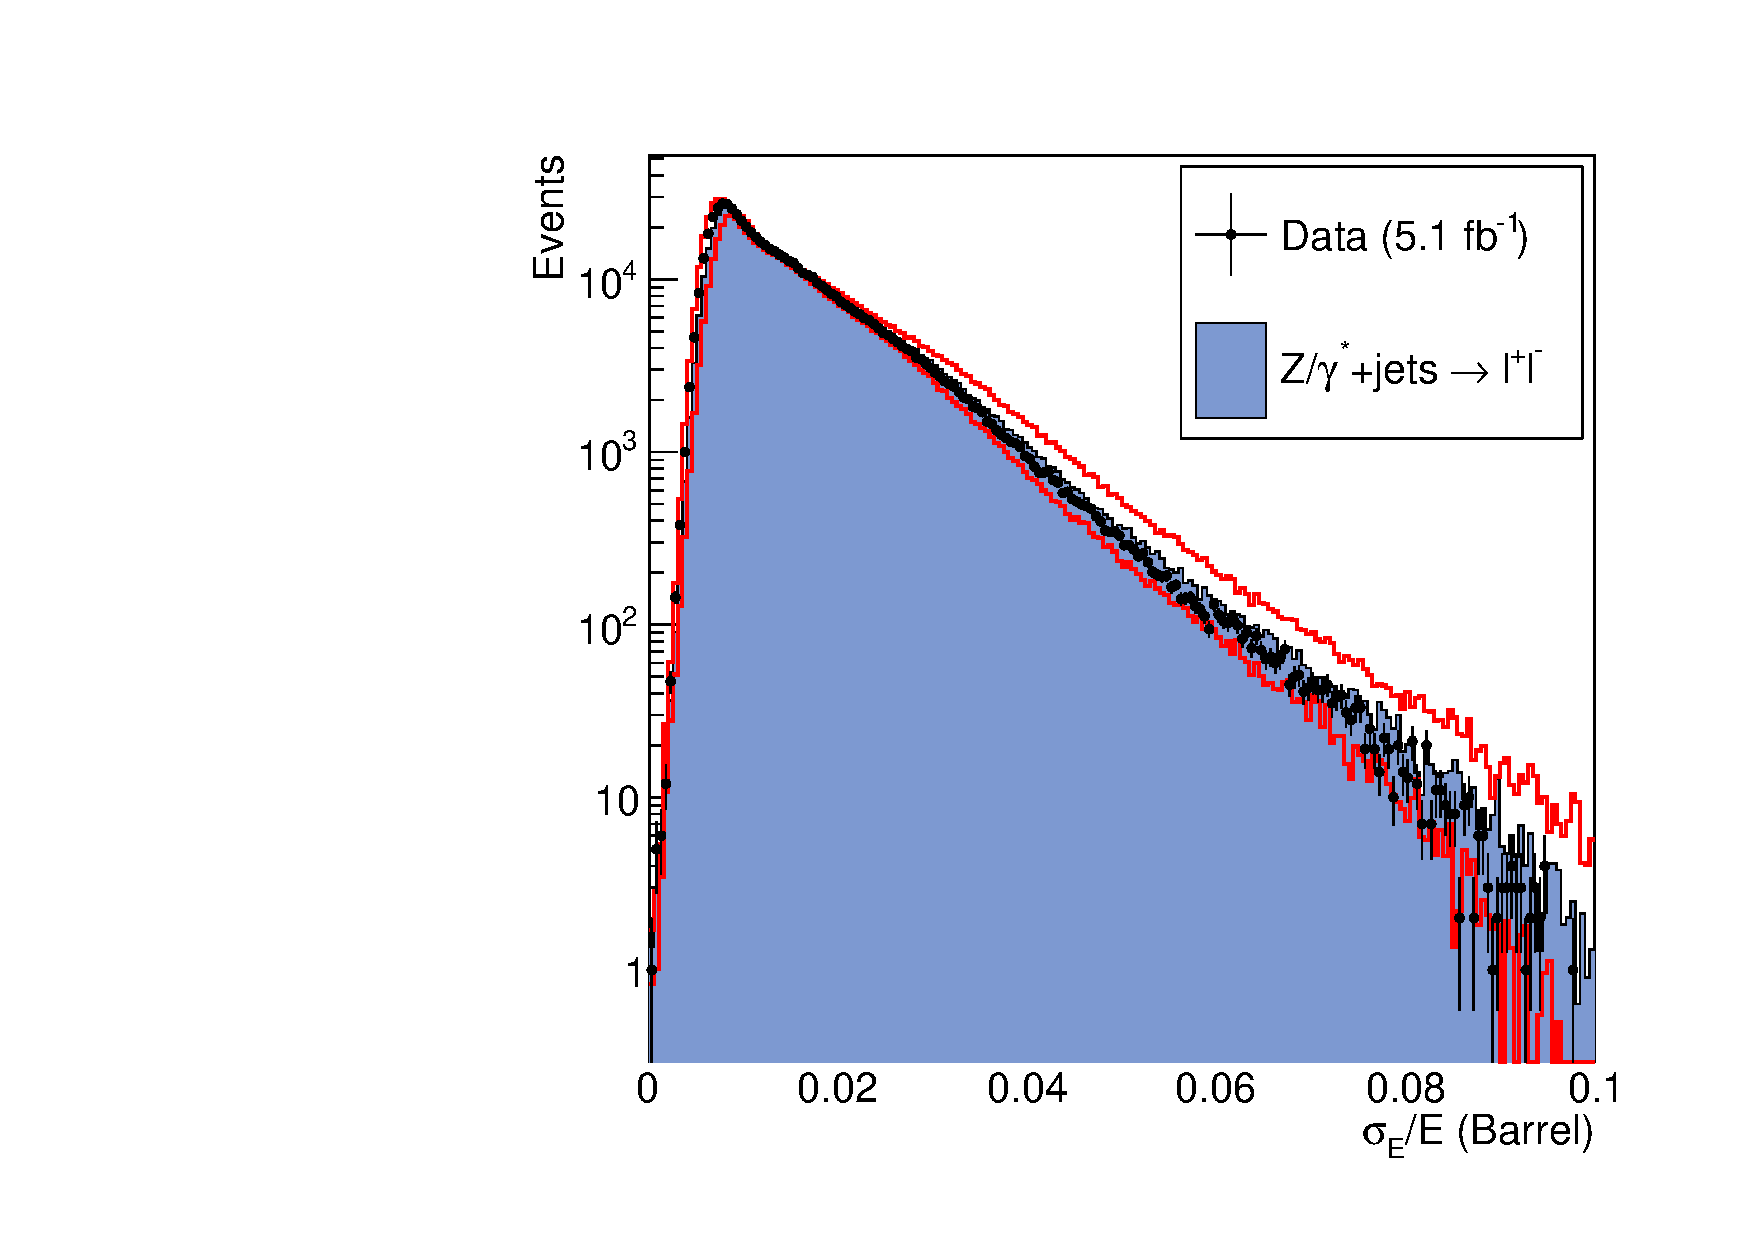
\includegraphics[width=.48\textwidth]{hgg7TeV/zeeValidation/sigmaE_EB.pdf}
  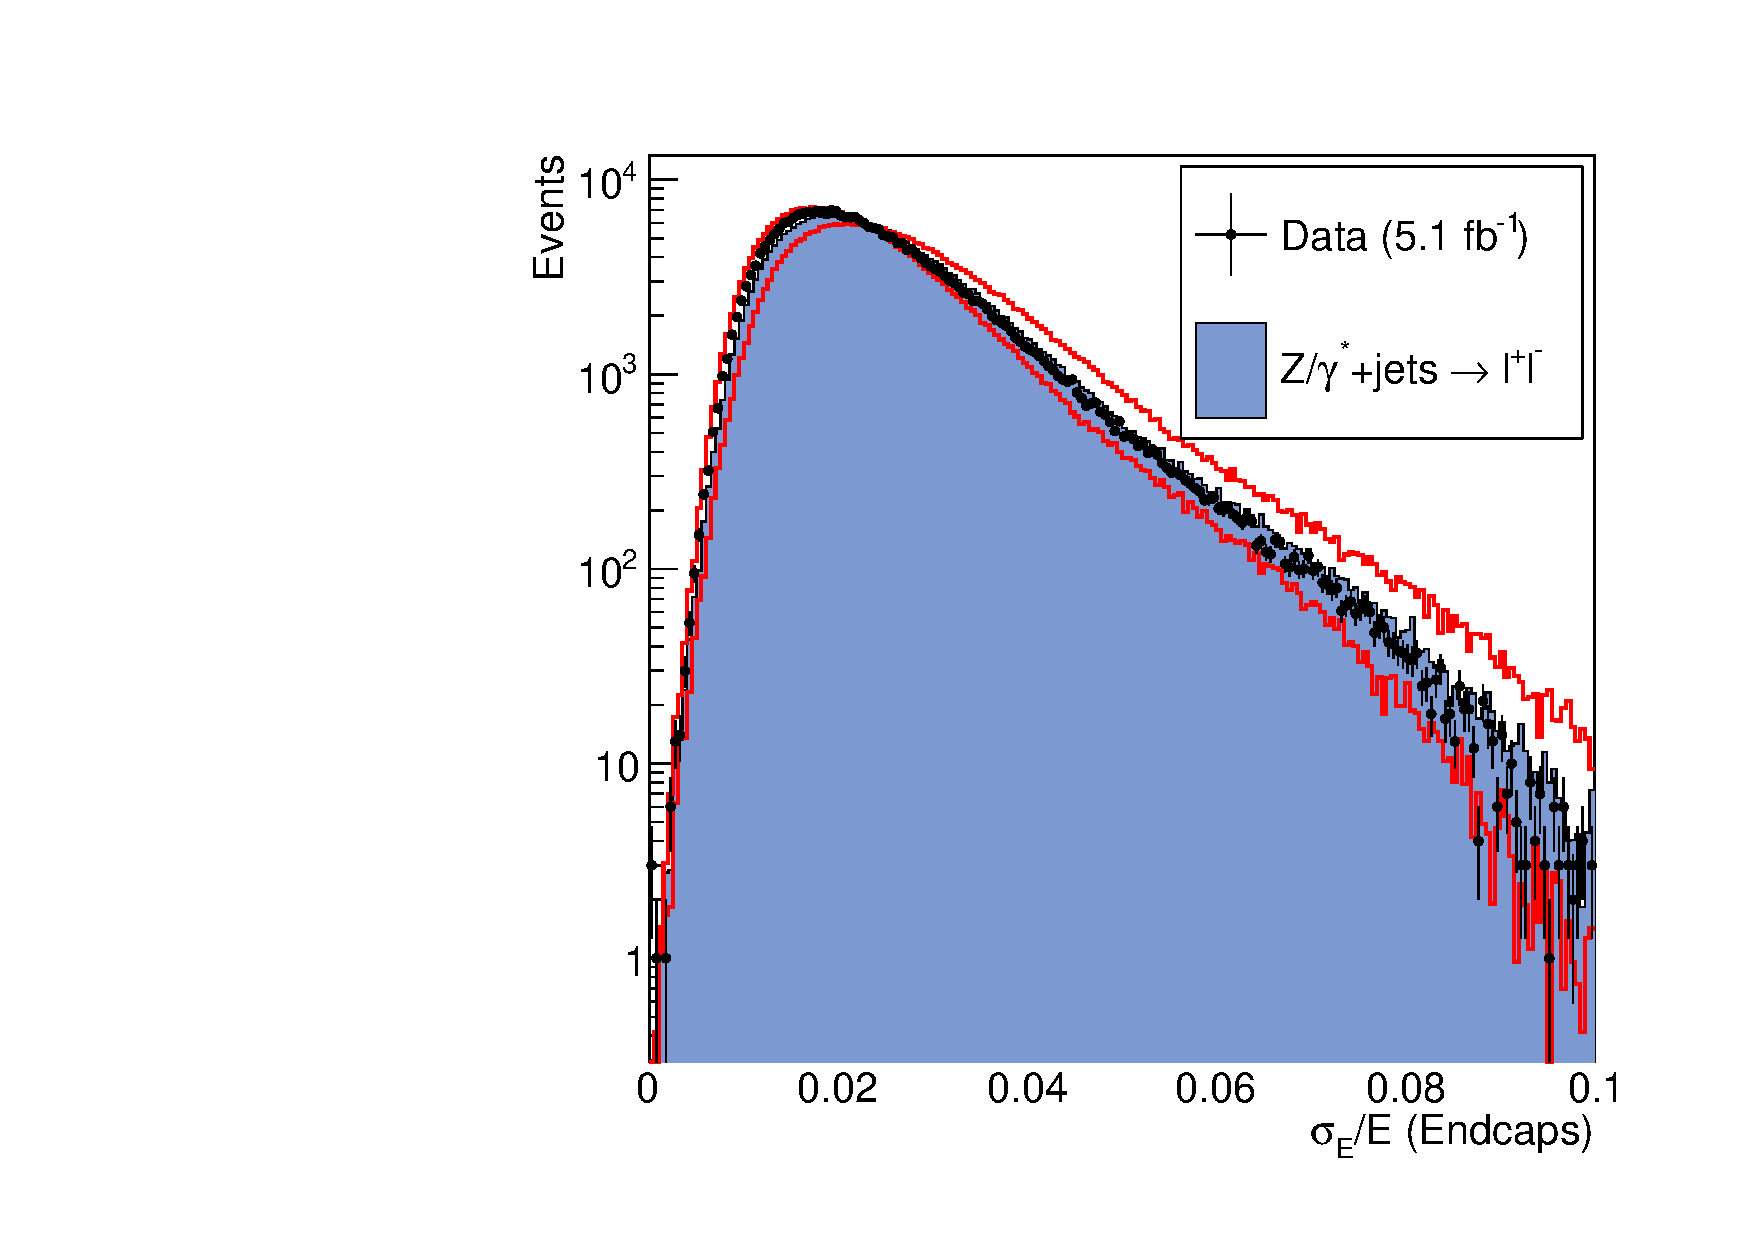
\includegraphics[width=.48\textwidth]{hgg7TeV/zeeValidation/sigmaE_EE.pdf}
\label{fig:zeevalidsigmaE}
\caption{Upper: Per-photon resolution estimator, $\sigma_{E}$ relative to the measured energy in $\Zee$ 
MC and data 
treating the electrons as photons in the barrel (left) and endcaps (right). 
The red lines show the $\pm 1\sigma$ systematic error envelope obtained by scaling the value of 
$\sigma_{E}$ by $\pm 10\%$.}
\end{center}
\end{figure}

\begin{figure}
\begin{center}
  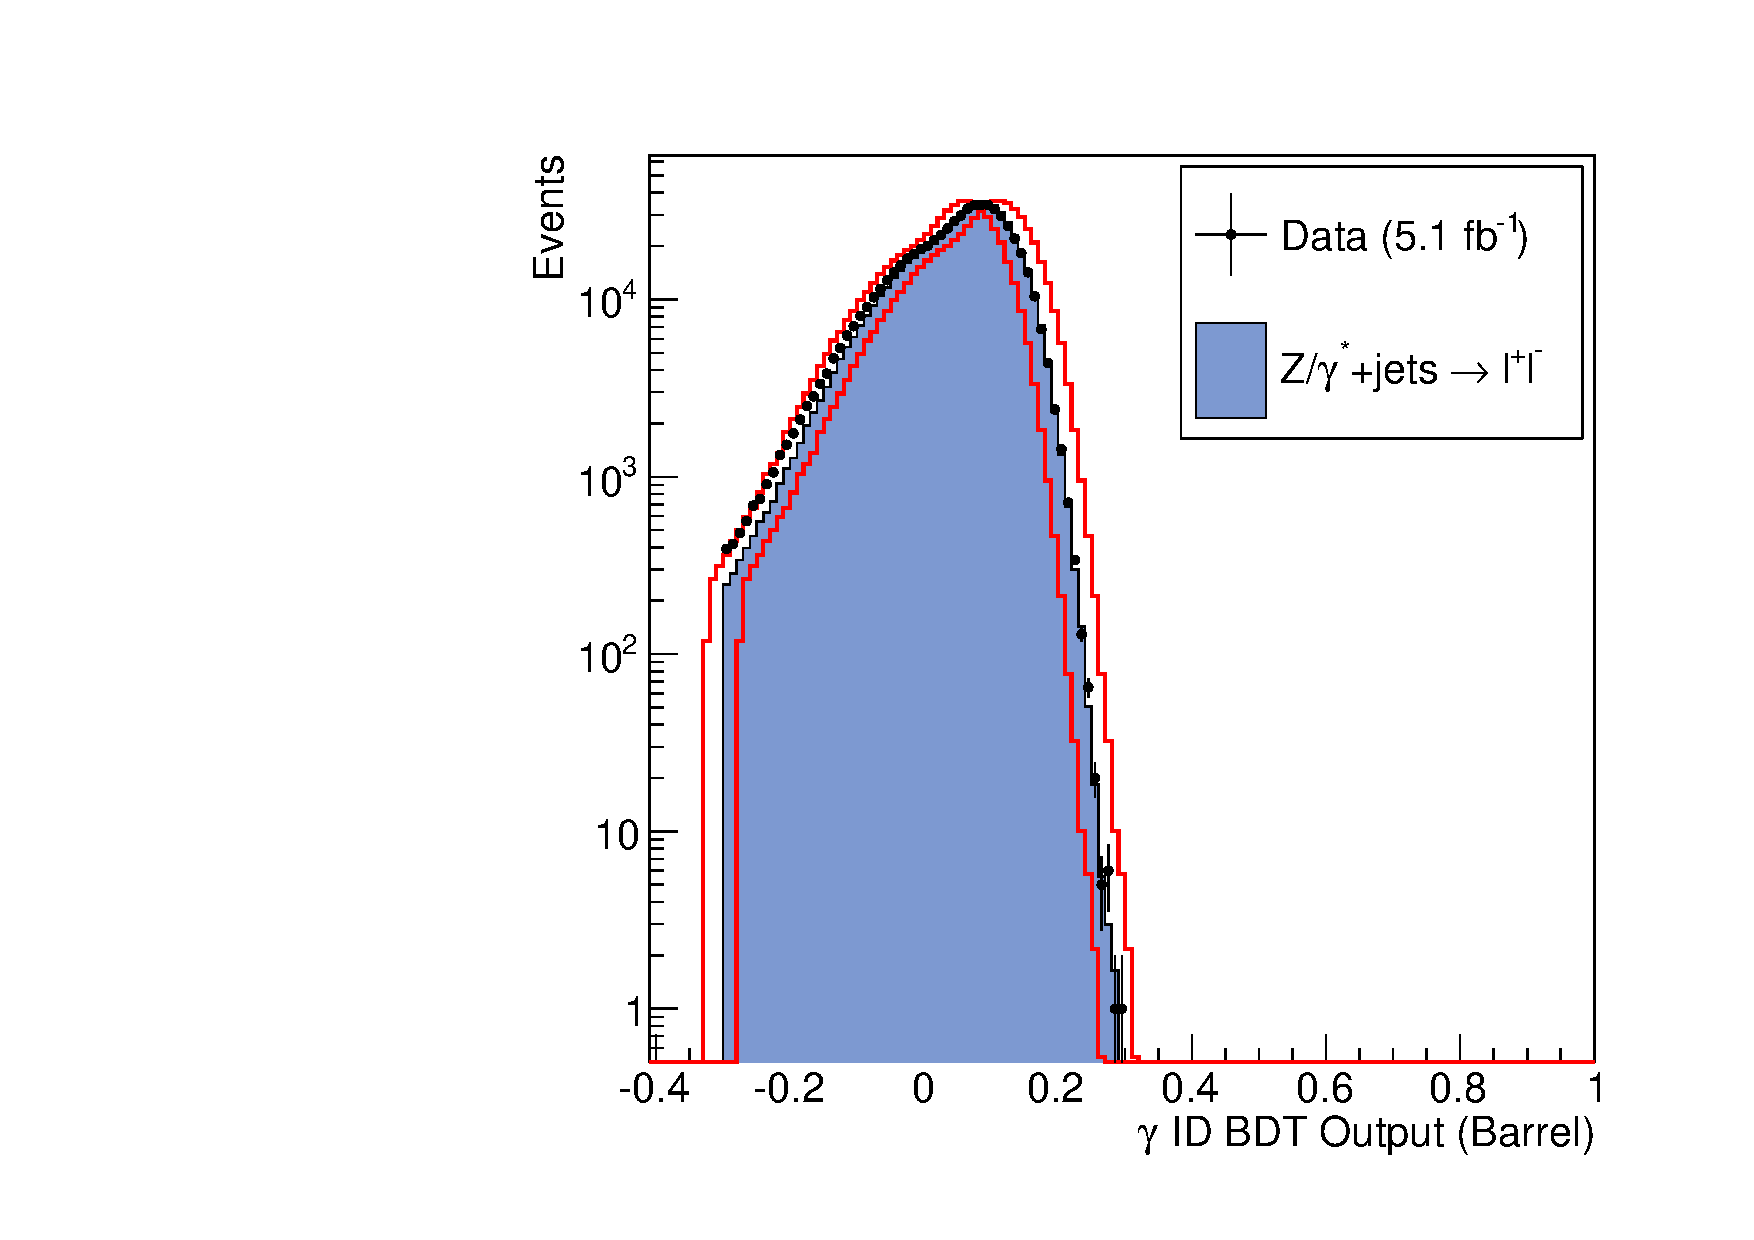
\includegraphics[width=.48\textwidth]{hgg7TeV/zeeValidation/phoID_EB.pdf}
  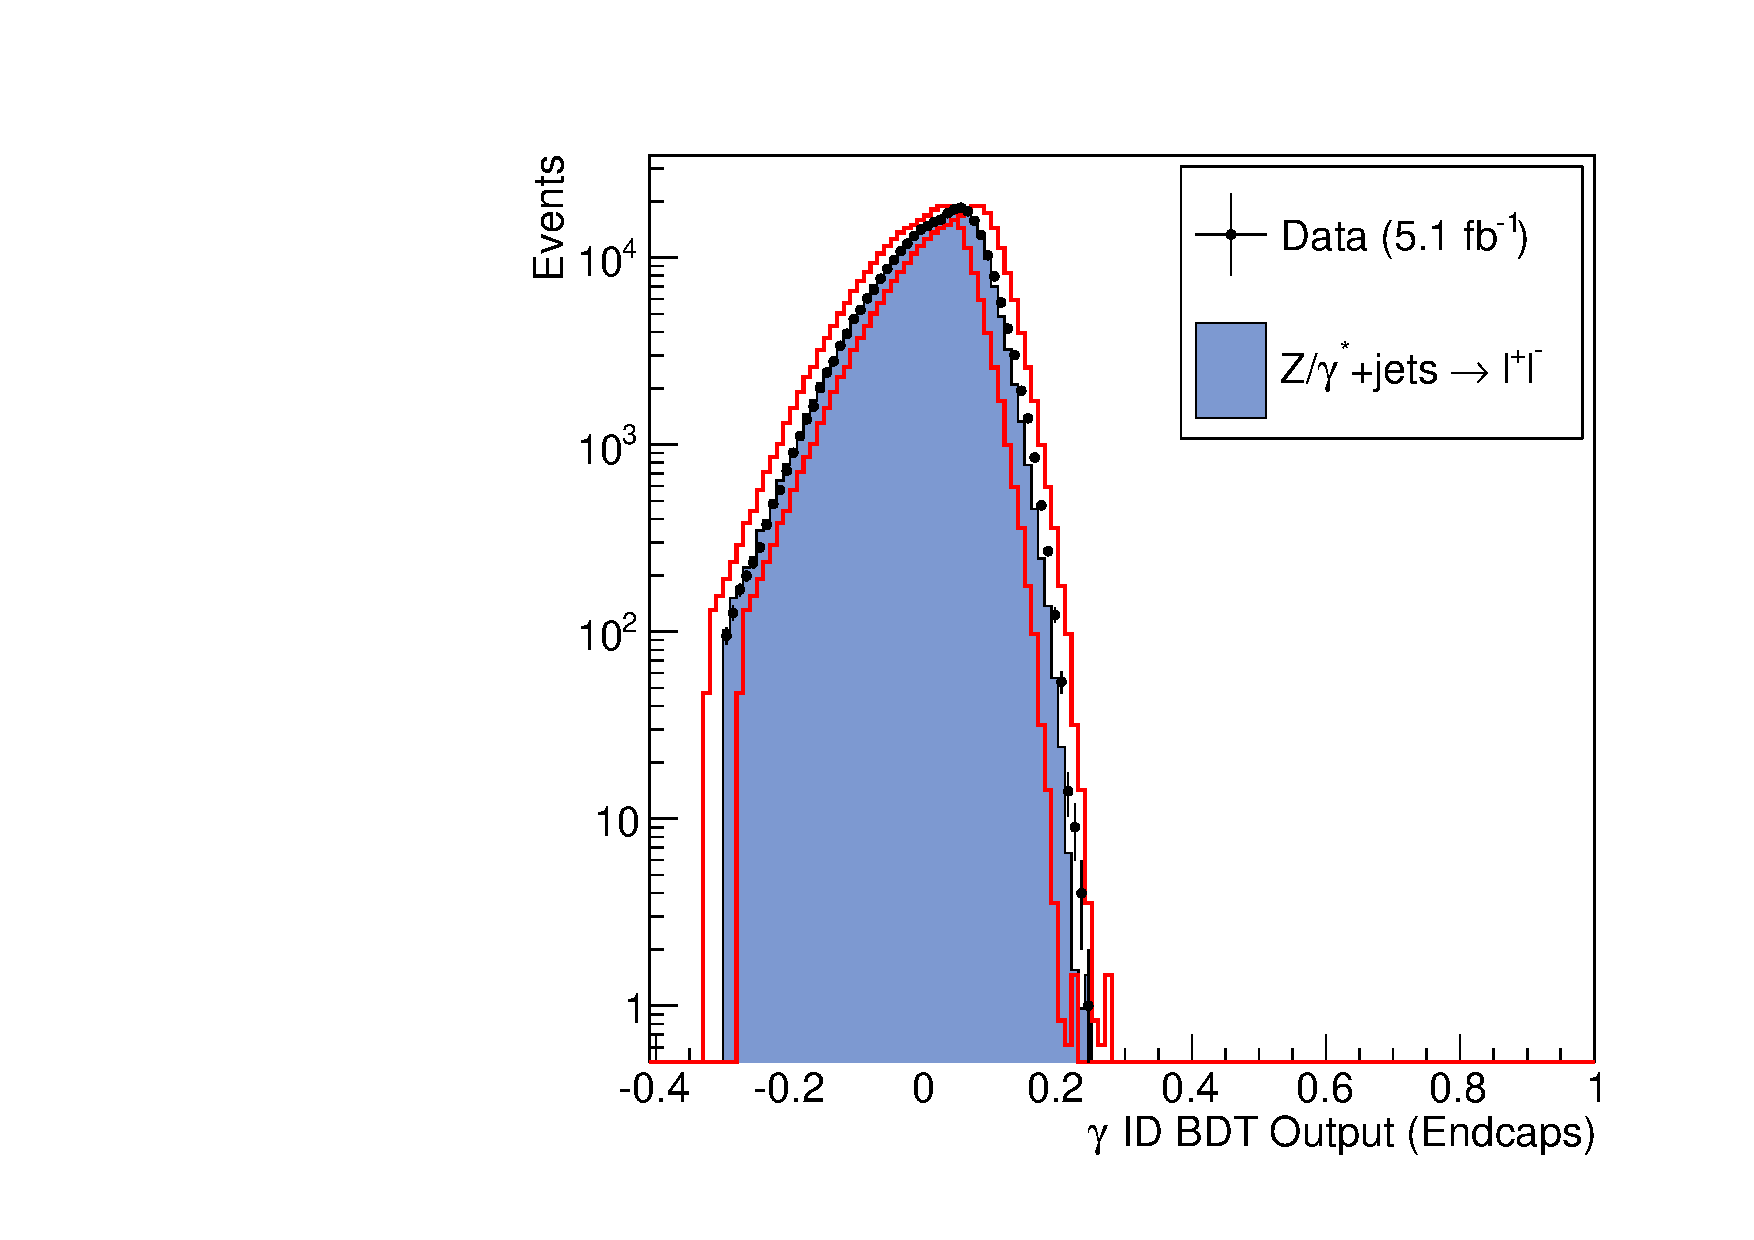
\includegraphics[width=.48\textwidth]{hgg7TeV/zeeValidation/phoID_EE.pdf}
\label{fig:zeevalidphoidmva}
\caption{Photon ID BDT output in $\Zee$ MC and data 
treating the electrons as photons in the barrel (left) and endcaps (right). 
The red lines show the $\pm 1\sigma$ systematic error envelope obtained by shifting the output value by $\sigma_{E}$ by $\pm 0.025\%$.}
\end{center}
\end{figure}


\subsection{Dijet Tagging}
\label{sec:dijettagging}

The contribution to Higgs production from vector boson fusion is around a factor ten smaller than that
of gluon-gluon fusion. However, additional information from the two jets associated 
with $qqH$ production allows for further reduction of the diphoton background~\ref{HIG-11-033}.
Events containing two jets which pass the full selection and in addition
satisfy a series of criteria designed to target the specific topology of the dijet system are 
tagged as likely to have originated from $qqH$ production. For example, Figure~\ref{fig:vbfdeta} shows the 
separation in $\eta$ between the two jets. Signal events from vector boson fusion production are
more likely to have a large separation than those from background processes. The full set of 
criteria is given in Table~\ref{tab:vbfcuts}.
The dijet tagged events are categorized separately to 
the remaining events, thereby exploiting their high signal to background ratio for the purpose of signal
extraction. 

\begin{table}
\begin{tabular}{|l|c|}
\hline
\textbf{Variable} & \textbf{Cut Value} \\
\hline
\hline
$E_{T}^{j^{1}}$ & $>$ 30 GeV \\
$E_{T}^{j^{2}}$ & $>$ 20 GeV \\
$m_{jj}$ 	 & $>$ 350 GeV \\
$|\eta_{j^{1}} - \eta_{j^{2}}|$ & $>$ 3.5 \\
$|\phi_{jj} - \phi_{\gamma\gamma}$ & $>$ 2.6 \\
$|0.5(\eta_{j^{1}} + \eta_{j^{2}}) - \eta_{\gamma\gamma}|$ & $<$ 2.5 \\
\hline
\end{tabular}
\label{tab:vbfcuts}
\caption{Dijet selection criteria for the two identified jets
to be considered likely associated to $qqH$ production. The leading and subleading $E_{T}$ jets
are denoted $j^{1}$ and $j^{2}$ respectively.}
\end{table}

\begin{figure}
\begin{center}
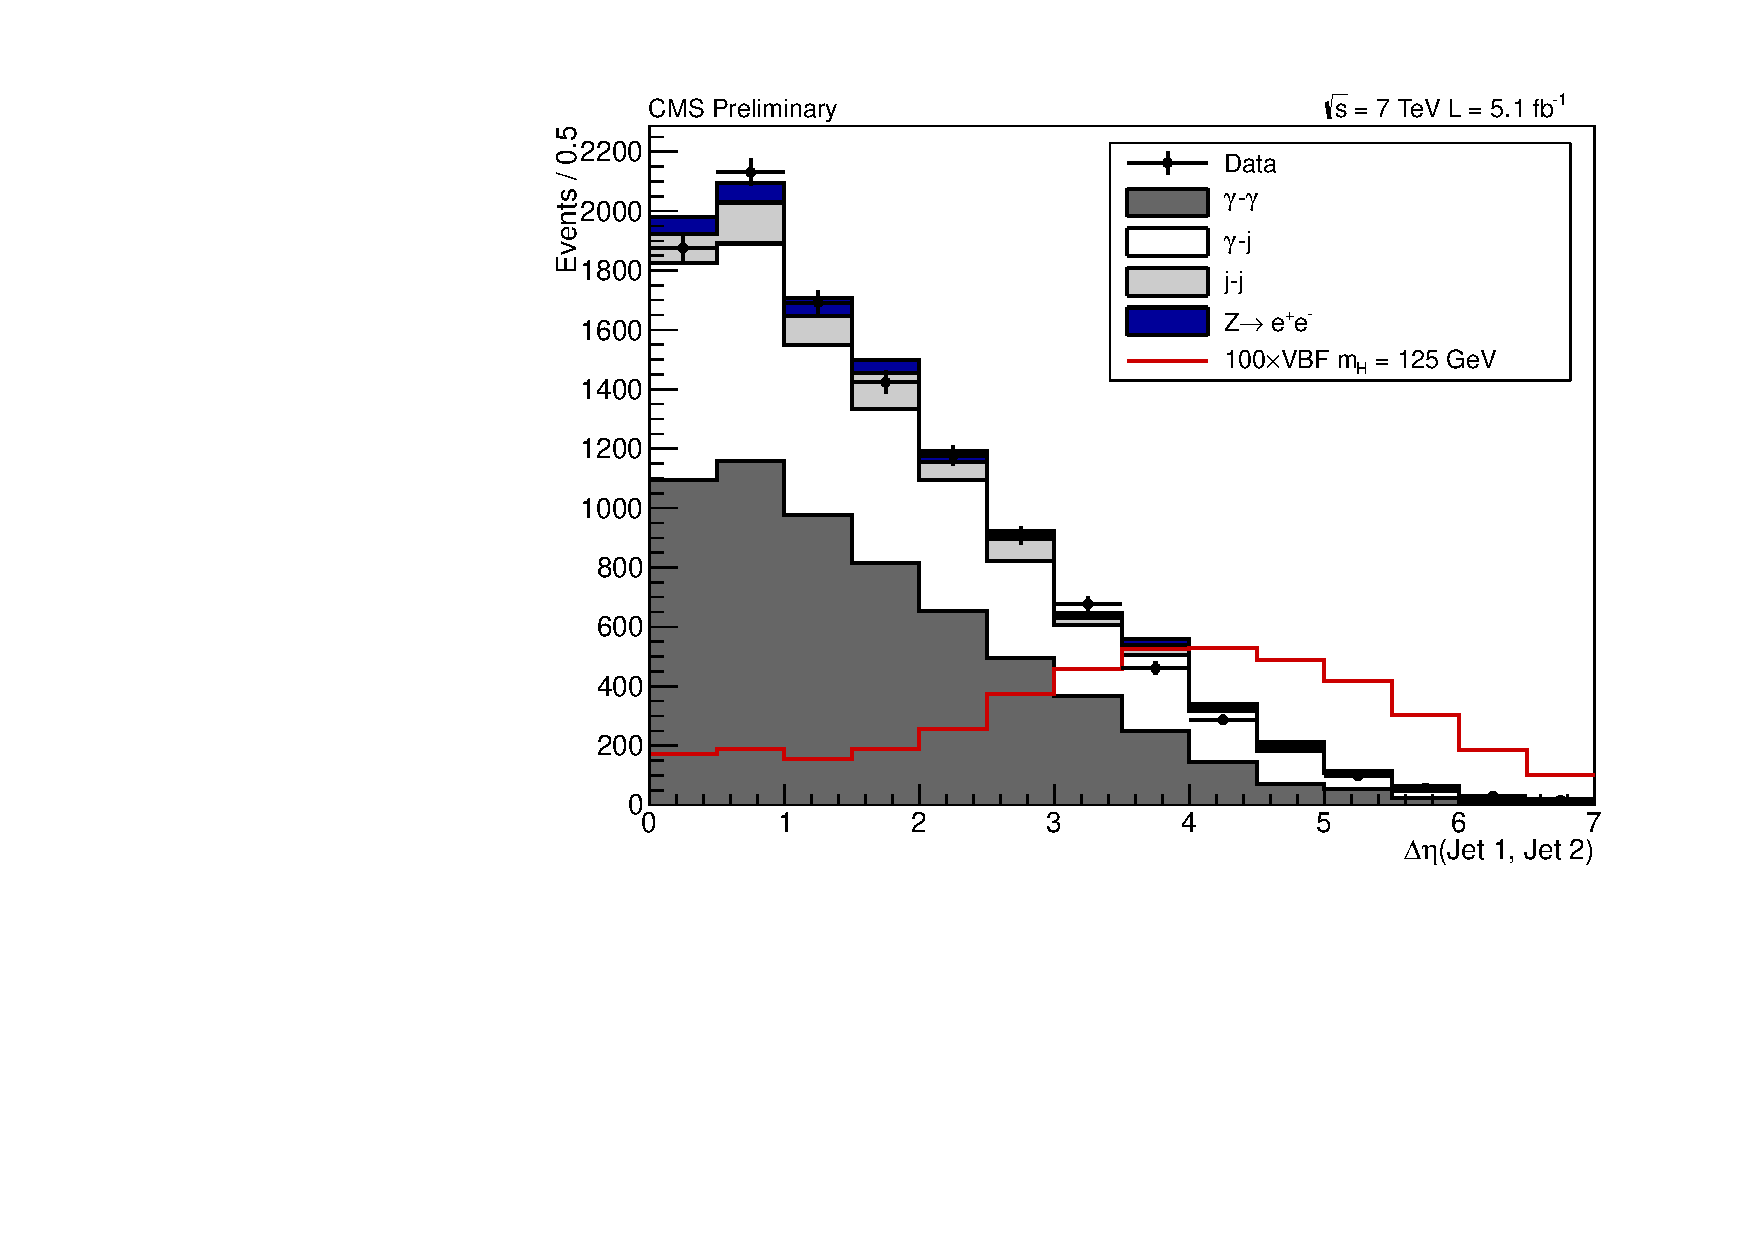
\includegraphics[width=0.8\textwidth]{hgg7TeV/variablePlots/cut_VBF_dEta_sequential_cat0.pdf}
\label{fig:vbfdeta}
\caption{Separation in $\eta$ between two identified jets in data and MC. 
The expectation from a SM Higgs produced via vector boson fusion ($qqH$), scaled by 100,
is shown in red. All cuts other than the one on $\Delta\eta(Jet 1, Jet2)$ are applied to these distributions.} 
\end{center}
\end{figure}

